\documentclass{createspace}
\newcommand{\N}{\mathbb N}
\newcommand{\Z}{\mathbb Z}
\newcommand{\Q}{\mathbb Q}
\newcommand{\R}{\mathbb R}
\newcommand{\C}{\mathbb C}

\newcommand{\shrap}{\mathbin{\#}}
\DeclareMathOperator*{\bigshrap}{\#}

\newcommand{\bracket}[1]{\left\langle{#1}\right\rangle}

\newcommand{\alexander}{\Delta}
\newcommand{\conway}{\nabla}
\newcommand{\jones}{V}
% span?

\newcommand{\braid}{\operatorname{b}}
\newcommand{\bridge}{\operatorname{br}}
\newcommand{\crossing}{\operatorname{cr}}
\newcommand{\genus}{\operatorname{g}}
\newcommand{\linking}{\operatorname{lk}}
\newcommand{\ropelength}{\operatorname{len}}
\newcommand{\sign}{\operatorname{sgn}}
\newcommand{\stick}{\operatorname{s}}
\newcommand{\unknotting}{\operatorname{u}}
\newcommand{\volume}{\operatorname{vol}}
\newcommand{\writhe}{\operatorname{wr}}

\newcommand{\inversedcurvearrowright}{\rotatebox[origin=c]{180}{$\curvearrowleft$}}
\newcommand{\inversedcurvearrowleft}{\rotatebox[origin=c]{180}{$\curvearrowright$}}
\newcommand{\MalyNieWezel} {\begin{tikzpicture}[baseline=-0.65ex, scale=0.02]
	\begin{knot}[clip width=5, end tolerance=1pt]
		\strand[semithick] (0,0) circle (5);
	\end{knot}
\end{tikzpicture}}

\newcommand{\NieWezel} {\begin{tikzpicture}[baseline=-0.65ex, scale=0.04]
	\begin{knot}[clip width=5, end tolerance=1pt]
		\strand[semithick] (0,0) circle (5);
	\end{knot}
\end{tikzpicture}}

\tikzset{
	->-/.style={decoration={markings, mark=at position .5 with {\arrow{>}}},postaction={decorate}},
	-<-/.style={decoration={markings, mark=at position .5 with {\arrow{<}}},postaction={decorate}},
	LUK/.style ={
		draw=black,
		line join=miter,
		line cap=butt,
		miter limit=4.00,
		line width=0.2 mm
	},
	CIENKILUK/.style ={
		draw=black,
		line join=miter,
		line cap=butt,
		miter limit=4.00,
		line width=0.1 mm
	},
	TEKSTOWY/.style ={
		draw=black,
		line join=round,
		line cap=butt,
		miter limit=20.00,
		line width=0.2 mm
	},
	OBSZAR/.style={
		draw=none,
		fill=white!#1!red
	},
	OBSZAR/.default = 80,
}

\usepackage{enumitem}
\usepackage{booktabs}
\usepackage{longtable}
\usepackage[table]{xcolor}
\usepackage[colorinlistoftodos,prependcaption]{todonotes}
\usepackage{tikz}
\usetikzlibrary{arrows.meta}
\usetikzlibrary{decorations.markings}
\usetikzlibrary{decorations.pathreplacing}
\usetikzlibrary{knots}
\colorlet{darkblue}{blue!80!black}

\author{Leon Suwalski}
\title{Krótkie wprowadzenie do teorii węzłów}
\date{2018}

\begin{document}
\maketitle
\tableofcontents
\chapter{Preludium}
\label{cha:preludium}
Teoria węzłów to gałąź topologii,
która powstała z~inspiracji węzłami,
jakie pojawiają się w~codziennym życiu: przy wiązaniu butów albo cumowaniu statków.
Zajmuje się ona badaniem przede wszystkim węzłów,
czyli pewnych włożeń okręgu $S^1$ w~trójwymiarową przestrzeń euklidesową $\R^3$ lub sferę $S^3$,
ale także splotów (zaplątanych w~sobie węzłów), warkoczy, supłów oraz podobnych obiektów.
Matematyczne węzły różnią się tym od zwykłych, że ich końce są ze sobą połączone.

Oto kilka przykładów.
Węzeł (a) nazywamy niewęzłem (jest to kalka angielskiego \emph{unknot}).
Następne w~kolejce widoczne są trójlistnik (b,~\emph{trefoil}), ósemka (c,~\emph{figure-eight}), pięciolistnik (d,~\emph{cinquefoil}) oraz słynna para Perko (e,~f~wg oryginalnej numeracji Rolfsena).

\begin{figure}[H]
    \centering
    \begin{minipage}[b]{.14\linewidth}
        \centering
        $\begin{tikzpicture}[baseline=-0.65ex, scale=0.5] \begin{knot}[clip width=5, end tolerance=1pt] \strand[semithick] (0,0) circle (\linewidth); \end{knot}
\end{tikzpicture}$
        \subcaption{}
    \end{minipage}
    \begin{minipage}[b]{.14\linewidth}
        \centering
        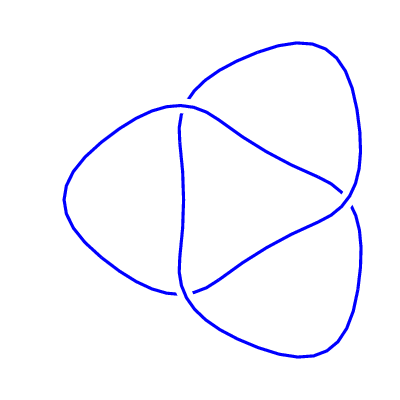
\includegraphics[width=\linewidth]{../data/3_1.png}
        \subcaption{$3_1$}
    \end{minipage}
    \begin{minipage}[b]{.14\linewidth}
        \centering
        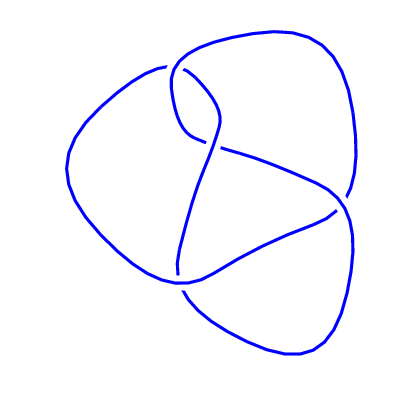
\includegraphics[width=\linewidth]{../data/4_1.png}
        \subcaption{$4_1$}
    \end{minipage}
    \begin{minipage}[b]{.14\linewidth}
        \centering
        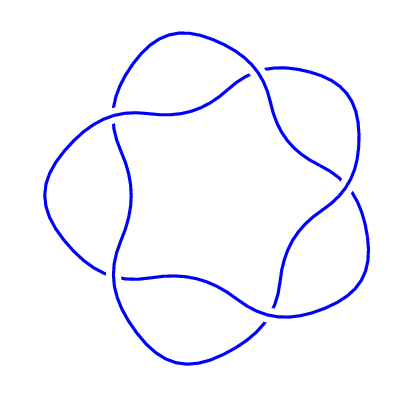
\includegraphics[width=\linewidth]{../data/5_1.png}
        \subcaption{$5_1$}
    \end{minipage}
    \begin{minipage}[b]{.14\linewidth}
        \centering
        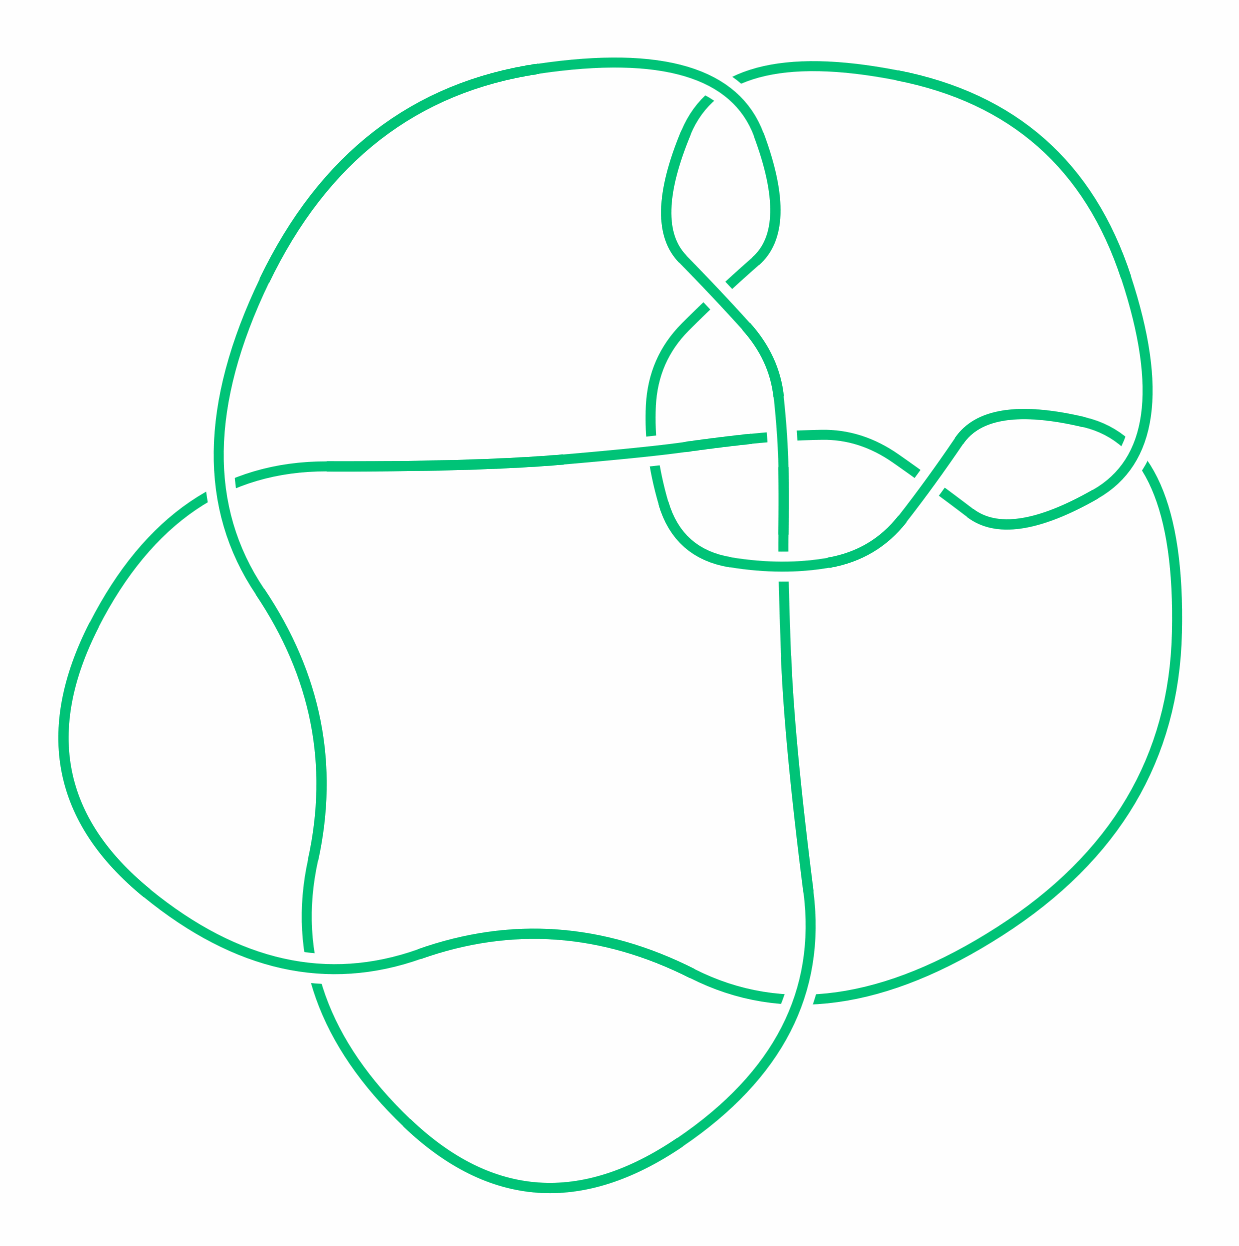
\includegraphics[width=\linewidth]{../data/perko1.png}
        \subcaption{$10_{161}$}
    \end{minipage}
    \begin{minipage}[b]{.14\linewidth}
        \centering
        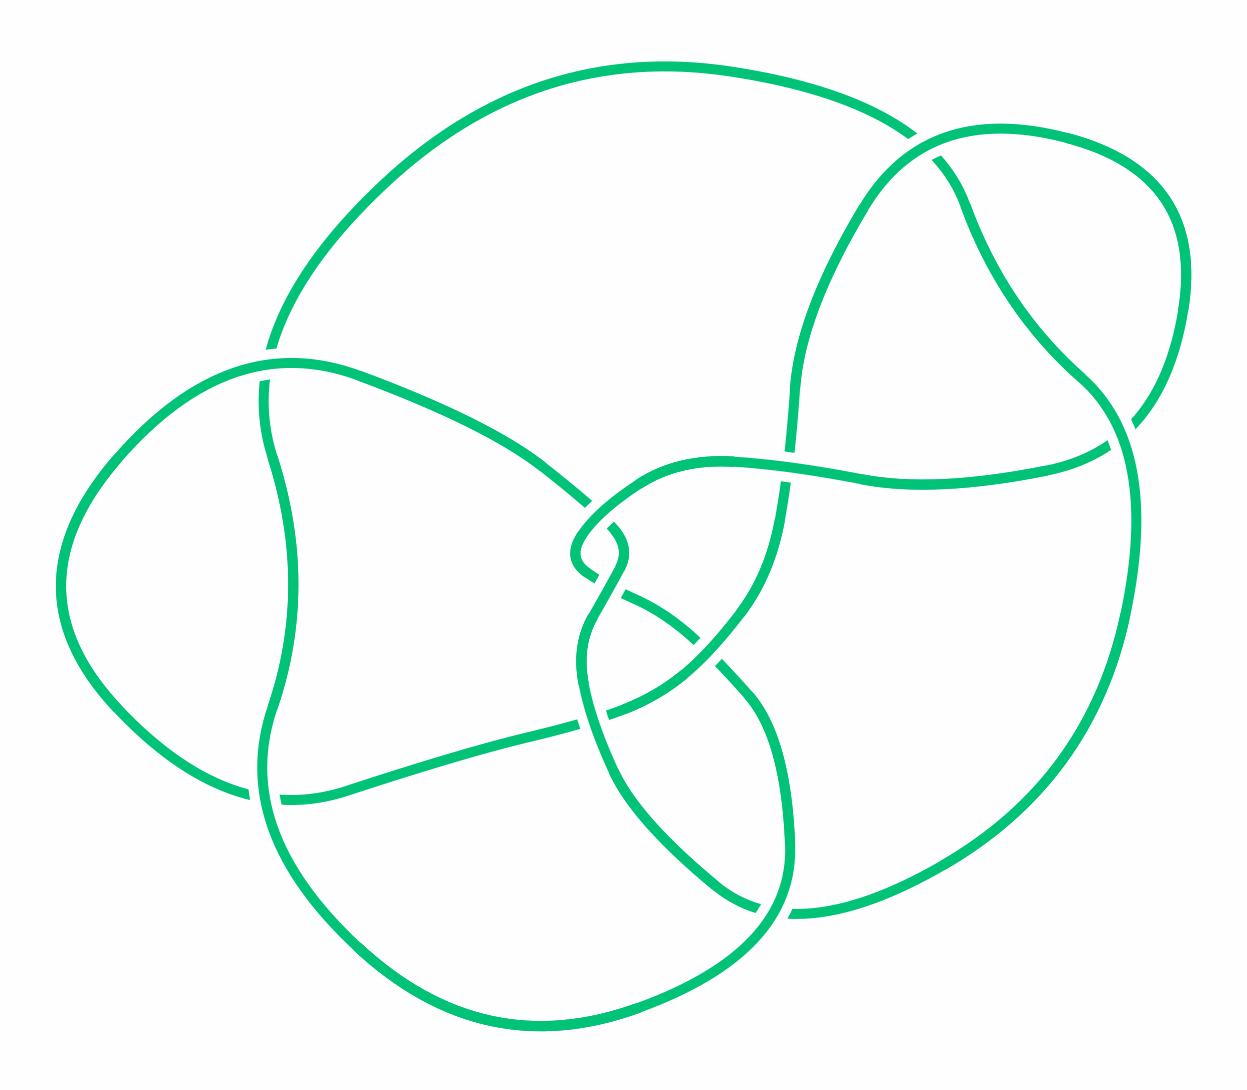
\includegraphics[width=\linewidth]{../data/perko2.png}
        \subcaption{$10_{162}$}
    \end{minipage}
\end{figure}

Początkowo celem teorii węzłów była klasyfikacja wszystkich węzłów.
Od XIX wieku, kiedy teoria węzłów wyodrębniła się jako osobny dział matematyki,
zdążyliśmy skatalogować ponad sześć miliardów tych obiektów.
Pozornie tak samo wyglądające węzły mogą się od siebie różnić.
Do wykrywania tych subtelnych różnic używa się przede wszystkim niezmienników topologicznych takich jak grupy, wielomiany bądź liczby.
Poznamy je w~dalszych rozdziałach.

Matematycy uogólnili pojęcie węzła:
można rozpatrywać je w~wyższych wymiarach albo zastąpić okrąg inną przestrzenią topologiczną.
Będziemy starać się unikać tych uogólnień.

\section{Węzły i~sploty}
Największą różnicą między węzłami matematycznymi oraz tymi z~prawdziwego jest życia jest to, że te pierwsze nie mają luźnych końców.
Można przyjąć nieidealną, naiwną definicję:

\begin{definition}[węzeł?]
    Ciągłe oraz różnowartościowe odwzorowanie $S^1 \to \R^3$ nazywamy węzłem.
\end{definition}

Zastanówmy się, jakim formalizmem opisać manipulowanie fizycznym sznurkiem.
Nie można użyć izotopii
(dwa węzły są izotopijne, jeśli istnieje ciągła funkcja $F \colon S^1 \times [0, 1] \to \R^3$ taka, że $F(-, 0)$ jest pierwszym, zaś $F(-,1)$ drugim węzłem).
Zauważmy, że każde splątanie ściąga się do punktu.
Dowolny węzeł jest równoważny z~trywialnym, zatem istnieje tylko jedna klasa abstrakcji.
Trzeba uwzględnić to, jak węzeł leży w~przestrzeni.
Właściwym narzędziem jest więc izotopia otaczająca.
Intuicyjnie: dwa węzły uznajemy za równoważne,
jeśli można przejść od jednego do drugiego przy użyciu deformacji całej przestrzeni $\R^3$.

\begin{definition}[izotopia otaczająca] \label{def_ambient_isotopy}
    Ciągłe odwzorowanie $F \colon \R^3 \times [0,1] \to \R^3$,
    które staje się homeomorfizmem po ustaleniu drugiego argumentu i~takie,
    że $F(-, 0)$ jest funkcją tożsamościową,
    zaś $F(-, 1)$ złożona z~pierwszym węzłem daje drugi węzeł,
    nazywamy izotopią otaczającą.
\end{definition}

\begin{definition}[węzeł]
    \label{def:knot}
    \index{węzeł}
    Gładkie włożenie $S^1 \to \R^3$ izotopijne otaczająco z~zamkniętą łamaną bez samoprzecięć nazywamy węzłem poskromionym.
\end{definition}

Wykluczamy w~ten sposób patologiczne z~kombinatorycznego punktu widzenia węzły dzikie.
Przez prawie całą książkę interesować nas będą jedynie węzły poskromione,
dlatego jeśli nie zaznaczono inaczej, przez węzeł rozumiemy węzeł poskromiony.

\begin{figure}
    \centering
    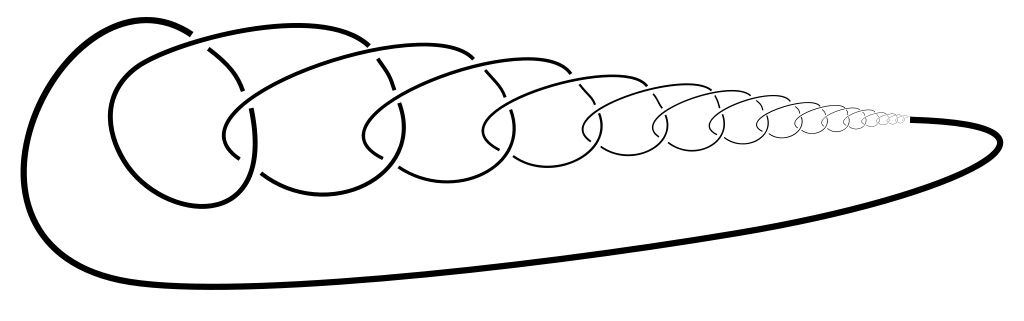
\includegraphics[width=0.5\linewidth]{wild_knot.png}
    \caption{Węzeł dziki}
\end{figure}

Dość często będziemy utożsamiać węzeł z~jego obrazem.

Jednocześnie homeomorfizmy $F(-,t)$ zastępujemy przez dyfeomorfizmy zachowujące orientację.
Chwila namysłu wystarcza do przekonania się, że definicja \ref{def_ambient_isotopy} obejmuje zwykłą izotopię,
a przy tym nie pozwala na rozwiązanie nietrywialnych węzłów przez ściągnięcie zaplątania do punktu.
Istnieje jeszcze jedna, konkurencyjna definicja węzłów równoważnych:

\begin{definition}
    \label{equivalent_knots_2}
    Dwa węzły są równoważne, gdy jeden z~nich jest obrazem drugiego przez zachowujący orientację homeomorfizm $\R^3 \to \R^3$.
\end{definition}

Stwierdzenie to przestaje być prawdziwe po zastąpieniu przestrzeni $\R^m$ przez $S^m$.

\begin{proof}
    Podany niżej dowód pochodzi z~książki ,,Topology from the differentiable viewpoint'' Johna Milnora.
    Musimy pokazać, że dyfeomorfizm $f \colon \R^m \to \R^m$ jest gładko izotopijny z~identycznością.
    Translacje są izotopiami, więc bez straty ogólności zakładamy, że $f(0) = 0$.
    Pochodna $f$ w~zerze jest dana wzorem $\mathrm{d}f_0(x) = \lim_{t \to 0} f(tx) /t$,
    naturalną definicją    izotopii $F \colon \R^m \times [0, 1] \to \R^m$ jest więc
    \[
        F(x, t) = \begin{cases}
            f(tx) / t & 0 < t \le 1 \\
            \mathrm{d}f_0(x) & t = 0
        \end{cases} .
    \]

    Funkcja $F$ jest gładka,
    gdyż na mocy lematu Hadamarda funkcja $f$ zapisuje się jako suma $x_1 g_1(x) + \ldots + x_mg_m(x)$,
    gdzie funkcje $g_i$ są gładkie, co jakoś kończy dowód.
\end{proof}

\begin{definition}[splot]
    \label{def_link}
    \index{splot}
    Sumę rozłączną skończenie wielu węzłów nazywamy splotem.
\end{definition}

Podobnie jak dla węzłów mówimy, że dwa sploty są równoważne, jeśli jeden jest obrazem drugiego przez zachowujący orientację homeomorfizm $\R^3 \to \R^3$.
Wtedy obydwa sploty mają tyle samo składowych.

\begin{example}
    \index{splot!Hopfa}
    Whitehead w~1934 odkrył kontrprzykład do nieudanego dowodu hipotezy Poincarego.
    Był nim splot o~dwóch składowych przedstawiony na poniższym rysunku.
    Splot Hopfa to najprostszy splot nietrywialny, którym w~1931 r. zajmował się Heinz Hopf,
    topolog niemiecki, w~ramach badań nad tzw. rozwłóknieniem (Hopf fibration).

    \begin{figure}[H]
        \begin{minipage}[b]{.48\linewidth}
            \centering
            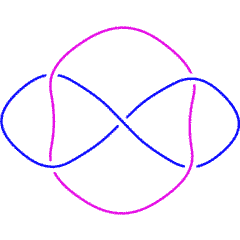
\includegraphics[width=0.5\linewidth]{../data/mixed/L5a1.png}
            \subcaption{splot Whiteheada}
        \end{minipage}
        \begin{minipage}[b]{.48\linewidth}
            \centering
            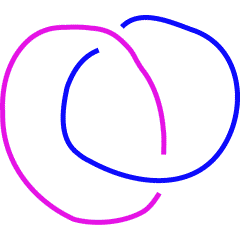
\includegraphics[width=0.5\linewidth]{../data/mixed/L2a1.png}
            \subcaption{splot Hopfa}
        \end{minipage}
    \end{figure}
\end{example}

\begin{definition}[rozszczepialność]
    \index{splot!rozszczepialny}
    Splot, który jest niespójną sumą niepustych splotów, nazywamy rozszczepialnym.
\end{definition}

Jeśli dwa węzły są równoważne, to ich dopełnienia są oczywiście homeomorficzne.
Pytanie o~prawdziwość implikacji odwrotnej jako pierwszy zadał najprawdopodobniej w~1908 roku Tietze (,,Über die topologischen Invarianten mehrdimensionaler Mannigfaltigkeiten'').
Od 1989 roku znamy odpowiedź na nie, jest pozytywna: każdy węzeł jest wyznaczony jednoznacznie przez swoje dopełnienie.
Wcześniej pokazano, że istnieją co najwyżej dwa węzły o~zadanym dopełnieniu.

\begin{theorem}[Gordon, Luecke, 1989] \label{thm_gordon_luecke}
    \index{twierdzenie!Gordona-Lueckego}
    Poskromione węzły o~homeomorficznych (z zachowaniem orientacji) dopełnieniach są wzajemnie izotopijne.
\end{theorem}

Twierdzenie to zamienia problem lokalny (czy dwa węzły w kuli $S^3$ są równoważne?) w~problem globalny (czy dwie przestrzenie topologiczne są homeomorficzne?).

\begin{proof}[Niedowód]
    Wynika to z~ogólniejszego stwierdzenia:
    nietrywialna chirurgia Dehna na węźle w~3-sferze nigdy nie daje 3-sfery.
    Pełny dowód zawiera praca \cite{gordon89}.
\end{proof}

Istnieje nieskończenie wiele (jakich?) kontrprzykładów do odpowiednika twierdzenia Gordona-Lueckego dla splotów,
których nie da się, patrząc na samo dopełnienie, odróżnić od splotu Whiteheada.

\section{Diagramy}
Chociaż w~świetle definicji \ref{def:knot} węzły są pewnymi regularnymi podzbiorami przestrzeni $\R^3$,
z kombinatorycznego punktu widzenia wygodniej jest rysować je na  płaszczyźnie.

\begin{definition} [diagram] \label{def_diagrams}
    \index{diagram}
    Cień to rzut węzła $K \subseteq \R^3$ na płaszczyznę.
    Diagram to cień bez katastrof
    (potrójnych przecięć, stycznych i~dziobów)
    razem z~informacją o~tym, jak przebiegają skrzyżowania.
\end{definition}

\begin{definition} [włókno]
    \index{włókno}
    Fragment diagramu, który biegnie między dwoma kolejnymi tunelami (podskrzyżowaniami) nazywamy włóknem.
\end{definition}

\begin{proposition}
    Każdy splot posiada diagram -- zbiór diagramów jest otwarty i~gęsty w~zbiorze wszystkich.
\end{proposition}

\begin{proof}
    Rzut splotu na równoległe płaszczyzny jest taki sam,
    a te można sparametryzować prostymi przechodzącymi przez początek układu współrzędnych,
    które tworzą przestrzeń rzutową $\R \mathbb P^2$.
    Niech $S$ będzie zbiorem prostych, które dają złe rzuty.
    Wystarczy pokazać jego nigdziegęstość.
    Okazuje się, że $S$ jest też jednowymiarowy.
    (Dowód za \cite{crowell63}).
\end{proof}

\begin{definition}
    \index{węzeł!alternujący}
    Diagram jest alternujący, gdy podczas poruszania się wzdłuż splotu mijamy jego skrzyżowania na zmianę z~góry oraz z~dołu.
    Splot jest alternujący, gdy posiada taki diagram.
\end{definition}

Nierozwiązanym problemem jest podanie definicji węzła alternującego, która nie odnosi się bezpośrednio do diagramów.
Sundberg oraz Thistlethwaite pokazali w 1998 roku, że liczba splotów alternujących rośnie wykładniczo (\cite{sundberg98}):

\begin{proposition}
    Niech $a_n$ oznacza liczbę pierwszych, alternujących supłów o~$n$ skrzyżowaniach.
    Wtedy
    \begin{equation}
        a_n \sim (3c_1/4\sqrt{\pi})n^{-5/2}\lambda^{n-3/2},
    \end{equation}
    gdzie zarówno $c_1$, pierwszy współczynnik rozwinięcia Taylora funkcji $\Phi(\eta)$ zdefiniowanej w \cite{sundberg98}, jak i $\lambda$ są jawnie znanymi stałymi:
    \begin{align}
        c_1 & = \sqrt{\frac{5^7 \cdot (21001 + 371 \sqrt{21001})^3}{2 \cdot 3^{10} \cdot (17 + 3\sqrt{21001})^5}} \\
        \lambda & = \frac {1}{40} (101 + \sqrt{21001})
    \end{align}
    Niech $A_n$ oznacza liczbę pierwszych, alternujących splotów o $n$ skrzyżowaniach.
    Wtedy $A_n \approx \lambda^n$, dokładniej: jeśli $n \ge 3$, to
    \begin{equation}
        \frac{a_{n-1}}{16n - 24} \le A \le \frac{a_n - 1}{2}.
    \end{equation}
\end{proposition}

Poniższy fakt stanowi jedynie szokującą ciekawostkę i także pochodzi z pracy \cite{sundberg98}.

\begin{proposition}
    Niech $a_n$ oznacza liczbę pierwszych, alternujących supłów o~$n$ skrzyżowaniach.
    Wtedy funkcja tworząca $f(z) = \sum_n a_n z^n$ spełnia równanie
    \begin{equation}
    f(1+z) - f(z)^2 - (1+f(z))q(f(z)) -z - \frac{2z^2}{1-z} = 0,
    \end{equation}
    gdzie $q(z)$ jest pomocniczą funkcją
    \begin{equation}
        q(z) = \frac{2z^2 - 10z - 1 + \sqrt{(1-4z)^3}} {2(z+2)^3} - \frac{2}{1+z} -z + 2.
    \end{equation}
\end{proposition}

%Niestety pomimo upływu czasus, nikt nie napisał komputerowego programu realizującego ten algorytm (stan na 1994).
%Może podejmie się tego Czytelnik?
%Inne algorytmy istnieją, jednak wszystkie działają w~wykładniczym czasie.

W 1961 roku W. Haken \cite{haken61} podał niezawodny przepis na wykrycie diagramu niewęzła,
częściowo rozwiązując jeden z~ważniejszych problemów teorii węzłów.
Przez wiele lat nikt nie podjął się implementacji tego algorytmu,
udało się to niedawno Burtonowi, Budneyowi oraz Petterssonowi w~komputerowym programie Regina\footnote{Dostępny pod adresem \url{https://regina-normal.github.io/}.} na przełomie tysiącleci.
Burton, Rubinstein i~Tillman pokazali w~pracy \cite{burton12}, jak sprawdzać,
czy powierzchnia normalna na striangulowanej 3-rozmaitości jest (nie)ściśliwa w~czasie wykładniczym.
To okazało się być wystarczającym do udzielenia negatywnej odpowiedzi na pytanie Thurstona:
,,czy przestrzeń Seiferta-Webera jest rozmaitością Hakena?'',
a zatem wykraczającego poza poziom tej pracy.
Patrz także {\url{http://geometrygames.org/SnapPea/index.html}.

Przykładami trudnych w~rozpoznaniu niewęzłów są: niewęzeł Goritza, Freedmana.

\begin{figure}[H]
    \begin{minipage}[b]{.32\linewidth}
        \centering
        
\includegraphics[width=\linewidth]{../data/missing.jpg}
        \subcaption{normalny}
    \end{minipage}
    \begin{minipage}[b]{.32\linewidth}
        \centering
        
\includegraphics[width=\linewidth]{../data/missing.jpg}
        \subcaption{Goritza}
    \end{minipage}
    \begin{minipage}[b]{.32\linewidth}
        \centering
        
\includegraphics[width=\linewidth]{../data/missing.jpg}
        \subcaption{Freedmana}
    \end{minipage}
\end{figure}

Więcej trudnych niewęzłów zawiera świeża praca
,,Algorithmic simplification of knot diagrams: new moves and experiments'
\footnote{\url{https://arxiv.org/pdf/1508.03226.pdf}}
C. Petronio, A. Zanellatiego.

\subsection{Historia tablic węzłów}
Pierwszą osobą, która podjęła się szukania węzłów, był Peter Guthrie Tait, szkocki fizyk.
Razem z Thomsonem (lordem Kelvinem) wierzyli, że węzły są kluczem do zrozumienia widma spektroskopowego różnych pierwiastków: na przykład atom sodu mógł być splotem Hopfa ze względu na dwie linie emisyjne.
Eksperyment Michelsona-Morleya z 1887 roku zabił ich ,,wirową teorię atomu'', ale nie miało to znaczenia dla teorii węzłów jako działu matematyki.

Używana po dziś dzień strategia, którą przyjął Tait, jest stosunkowa prosta: narysować wszysktie możliwe diagramy o~zadanym indeksie skrzyżowaniowym, po czym połączyć ze sobą te, które przedstawiają jeden węzeł.
Na potrzeby pierwszego etapu Tait wymyślił schemat kodowania diagramów.
Wiele lat wcześniej, Gauss wraz ze swoim uczniem Listingiem badał węzły i~opracował (niezależnie!) podobną notację.
My przytoczymy opis dalszego ulepszenia tej metody, zwanego notacją Dowkera-Thistletwaite’a.

Tait wykorzystując swoją notację podał w~1876 pierwszą tablicę piętnastu węzłów o~mniej niż ośmiu skrzyżowaniach.
Nie należy traktować tego jako skromny wynik: nie miał on do dyspozycji żadnych twierdzeń topologicznych do odróżniania węzłów.
Onieśmielony przez liczbę możliwych ciągów dla kolejnych indeksów skrzyżowaniowych, powstrzymał się przed rozszerzaniem swojej tablicy.
To właśnie grupowanie diagramów przedstawiających ten sam węzeł, a~nie samo szukanie wszystkich możliwych diagramów, sprawia trudność.

Aby sobie pomóc, Tait znalazł lokalną modyfikację diagramu, która nie zmienia indeksu skrzyżowaniowego, znaną obecnie jako flype.

\[
\begin{tikzpicture}[baseline=-0.65ex, scale=0.1]
\begin{knot}[clip width=5, end tolerance=1pt, flip crossing/.list={1}]
    \strand[semithick] (-21, -5) [in=180, out=0] to (-7, 5);
    \strand[semithick] (-21, 5) [in=180, out=0] to (-7, -5);
    \draw (-7, -7) rectangle (7, 7);
    \node at (0, 0) {\Huge {$T$}};
    \draw[semithick] (7, -5) to (21, -5);
    \draw[semithick] (7, 5) to (21, 5);
\end{knot}
\end{tikzpicture}
\quad \cong_{\mathrm{flype}} \quad
\begin{tikzpicture}[baseline=-0.65ex, scale=0.1]
\begin{knot}[clip width=5, end tolerance=1pt]
    \strand[semithick] (21, -5) [in=0, out=180] to (7, 5);
    \strand[semithick] (21, 5) [in=0, out=180] to (7, -5);
    \draw (-7, -7) rectangle (7, 7);
    \node at (0, 0) {\rotatebox[origin=c]{-180}{\Huge $T$}};
    \draw[semithick] (-7, -5) to (-21, -5);
    \draw[semithick] (-7, 5) to (-21, 5);
\end{knot}
\end{tikzpicture}
\]

Inną taktykę szukania węzłów przyjał wielebny Thomas Kirkman: zaczynał od małego zbioru "nieredukowalnych" rzutów, do których systematycznie dokładał skrzyżowania.
Tait przeczytał pracę Kirkmana, po czym w~latach 1884/1885 opracował listę węzłów alternujących o~mniej niż 11 skrzyżowaniach.
Tuż przed oddaniem jej do druku odkrył inny spis węzłów stworzony przez amerykańskiego naukowca Charlesa Little'a.
Znalazł wtedy jeden duplikat u~siebie, natomiast u Little'a jeden duplikat i~jedno pominięcie.

Zachęcony przez Taita, Little zabrał się za alternujące węzły o~11 skrzyżowaniach i~za trudniejsze zadanie, stablicowanie węzłów niealternujących, czyli takich, które nie posiadają alternującego diagramu.
Jak wynika z~pierwszej pracy Taita, początkowo nie wierzono, że takich w~ogóle nie ma.
Dowód istnienia znaleziono dopiero w~1930 roku, niealternujące są $8_{19}$, $8_{20}$, $8_{21}$, ale nie pierwsze węzły o mniejszej liczbie skrzyżowań.
Little pracował przez sześć lat (1893 -- 1899) i~znalazł 43 niealternujące węzły o~10 skrzyżowaniach.
Żadnego nie pominął, ale trafił mu się jeden duplikat.

W kolejnych dziesięcioleciach nie nastąpił znaczący postęp, zarówno w~rozszerzaniu tablic jak i~sprawdzaniu tych już istniejących.
Haseman w~1918 roku znalazł achiralne węzły o~12 i~14 skrzyżowaniach.
W 1927 roku Alexander z~Briggsem przy użyciu pierwszej grupy homologii rozgałęzionego nakrycia cyklicznego (!) potrafili odróżnić od siebie dowolne dwa węzły (z~pominięciem trzech par) o~co najwyżej 9 skrzyżowaniach.
Reidemeister poradził sobie z~tymi wyjątkami w~1932 roku, korzystając z~indeksu zaczepienia i~homomorfizmów z~grupy węzła na grupy diedralne.
% branch curves in irregular covers associated to homomorphisms of the knot group onto dihedral groups

%%%%% Tait, Little wyprodukowali prawie bezbłędną tablicę węzłów o~co najwyżej 11 skrzyżowaniach przy użyciu grafów.

Dopiero Conway w~latach sześćdziesiątych minionego wieku znalazł pierwsze węzły o~mniej niż 12 skrzyżowaniach oraz wszystkie sploty o~mniej niż 11 skrzyżowaniach w~oparciu o~pomysły Kirkmana.
% An enumeration of knots and links, 1970.
Zajęło mu to jedynie kilka godzin!
Conway znalazł 1 duplikat oraz 11 pominięć w~tablicach Little'a, ale sam popełnił 4 pominięcia.
Przeoczył między innymi słynny duplikat w~niealternującej tablicy Little'a, parę Perko.
% 1974?
Przyczyną było prawdopodobnie to, że dwa diagramy miały różny spin:
Little błędnie twierdził, że spin minimalnego diagramu jest niezmiennikiem, gdyż błędnie założył, że flype oraz 2-przejścia wystarczają do zmiany jednego minimalnego diagramu w~inny.

Pominęcia w~tablicy Conwaya znalazł Caudron w~1980 roku.
Nieopublikowany manuskrypt Bonahona, Siebenmanna klasyfikuje węzły algebraiczne.
Z~nielicznymi niealgebraicznymi węzłami do 11 skrzyżowań poradził sobie Perko około 1980 roku (,,Invariants of 11-crossing knots'').
To był kres ery ręcznych obliczeń.

Na początku lat osiemdziesiątych Dowker i~Thistlethwaite stabularyzowali z~pomocą komputera węzły do 13 skrzyżowań.
Przez blisko dekadę nic się nie działo, aż grupa studentów wygrała dostęp do superkomputera Cray.
Razem z~Hoste znaleźli alternujące węzły do 14 skrzyżowań, jednocześnie sprawdzając istniejące tabele Thistlethwaite'a.
Około roku 1998 Hoste z~Weeksem (oraz niezależnie Thistlethwaite) znaleźli 1701936 pierwszych węzłów do 16 skrzyżowań.
Spośród nich, tylko 32 nie jest węzłami hiperbolicznymi, wszystkie pozostałe poddają się maszynerii geometrii hiperbolicznej.

\subsection{Hipotezy Taita}
\begin{conjecture}[I hipoteza Taita]
    \label{conj_tait_i}
    \index{hipoteza!Taita}
    Zredukowany alternujący diagram splotu ma minimalny indeks skrzyżowaniowy.
\end{conjecture}
% To bardzo ważny rezultat, którego prawdziwość przypuszczał już P. G. Tait w~XIX wieku.
% Nikt nie był w~stanie podać dowodu przed pojawieniem się wielomianu Jonesa.

\begin{conjecture}[II hipoteza Taita]
    \label{conj_tait_ii}
    Achiralny splot alternujący ma zerowy spin.
\end{conjecture}

\begin{conjecture}[III hipoteza Taita]
    \label{conj_tait_iii}
    Niech $D_1, D_2$ będą zredukowanymi alternującymi diagramami zorientowanego pierwszego splotu.
    Wtedy diagram $D_2$ można otrzymać z~$D_1$ korzystając jedynie z~ruchu \emph{flype}.
\end{conjecture}

Z III hipotezy Taita wynika, że dwa zredukowane diagramy alternujące tego samego węzła mają ten sam spin: ruch flype nie zmienia spinu.
Bezpośredni dowód przeprowadzili Murasugi (1987) i Thistlethwaite (1988).
My pokażemy nieco później, czyli po poznaniu wielomianu Jonesa, że wszystkie trzy hipotezy są prawdziwe.

\subsection{Metody kodowania}
\subsubsection{Notacja Dowkera--Thistlethwaite'a}
Poprawia notację Taita.
Przypisuje ona (niejednocznacznie) każdemu węzłowi permutację znakowanych liczb parzystych $\pm 2, \pm 4, \ldots, \pm 2N$.

\subsubsection{Notacja Alexandera-Briggsa}
Najbardziej tradycyjna, wprowadzona w~1927 roku, rozszerzona później przez Rolfsena.

\subsubsection{Notacja Conwaya}
Wprowadzona przez Conwaya w~pracy \cite{conway70}.

% A pictorial enumeration of prime knots of up to 10 crossings appears in Rolfsen (1976, Appendix C).
% Note, however, that in this table, the Perko pair 10-161 and 10-162 are actually identical, and the uppermost crossing in 10-144 should be changed (Jones 1987).

% Rolfsen's last four 10 crossing knots have been renumbered, to avoid the Perko duplication.
% A further mistake in Rolfsen's tables is that therein 1083 and 1086 were swopped: the Conway notation and Alexander polynomial for each one referred to the diagram of the other.
% We exchange not diagrams, but Alexander polynomial and Conway notation to fix the mistake (like the table in the new 2003 edition of the Rolfsen book, Dror Bar-Natan's Knot Atlas, and Chuck Livingston's Table of Knot Invariants, and unlike in Kawauchi's book!).
% http://stoimenov.net/stoimeno/homepage/ptab/

\section{Ruchy Reidemeistera}
\label{sec:reidemeister_moves}
W kombinatorycznej teorii węzłów diagramy są dużo ważniejsze od gładkich włożeń okręgu w~przestrzeń $\R^3$,
dlatego przytoczymy proste kryterium decydujące o~tym,
kiedy dwa diagramy przedstawiają jeden węzeł.
Najpierw zdefiniujmy trzy lokalne operacje na diagramach.

\begin{definition}
    \index{ruchy Reidemeistera}
    Trzy ruchy Reidemeistera, $R_1$, $R_2$, oraz $R_3$, to następujące deformacje diagramu:
    \[
        \underbrace{\begin{tikzpicture}[baseline=-0.65ex,scale=0.1]
        \begin{knot}[clip width=5]
            \strand[thick] (-5, 10) to [in=left, out=down] (2, -5);
            \strand[thick] (5, 0) to [in=right, out=down] (2, -5);
            \strand[thick] (5, 0) to [in=right, out=up] (2, 5);
            \strand[thick] (-5, -10) to [in=left, out=up] (2, 5);
        \end{knot}
        \end{tikzpicture}
        \, \cong \,
        \begin{tikzpicture}[baseline=-0.65ex,scale=0.1]
        \begin{knot}[clip width=5]
            \strand[thick] (0,10) to (0,-10);
        \end{knot}
        \end{tikzpicture}}_{R_1}
        %%%
        \quad \quad \quad
        \underbrace{\begin{tikzpicture}[baseline=-0.65ex,scale=0.1]
        \begin{knot}[clip width=5]
            \strand[thick] (-5, 10) to [in=up, out=down] (5, 0);
            \strand[thick] (-5, -10) to [in=down, out=up] (5, 0);
            \strand[thick] (5, 10) to [in=up, out=down] (-5, 0);
            \strand[thick] (5, -10) to [in=down, out=up] (-5, 0);
        \end{knot}
        \end{tikzpicture}
        \, \cong \,
        \begin{tikzpicture}[baseline=-0.65ex,scale=0.1]
        \begin{knot}[clip width=5]
            \strand[thick] (-5, 10) to [in=up, out=down] (-2, 0);
            \strand[thick] (-5, -10) to [in=down, out=up] (-2, 0);
            \strand[thick] (5, 10) to [in=up, out=down] (2, 0);
            \strand[thick] (5, -10) to [in=down, out=up] (2, 0);
        \end{knot}
        \end{tikzpicture}}_{R_2}
        %%%
        \quad \quad \quad
        \underbrace{\begin{tikzpicture}[baseline=-0.65ex,scale=0.1]
        \begin{knot}[clip width=5, flip crossing/.list={1,2,3}]
            \strand[thick] (-10, -10) -- (10, 10);
            \strand[thick] (-10, 10) -- (10, -10);
            \strand[thick] (-10, 0) to [in=left, out=right] (0, 10);
            \strand[thick] (10, 0) to [in=right, out=left] (0, 10);
        \end{knot}
        \end{tikzpicture}
        \, \cong \,
        \begin{tikzpicture}[baseline=-0.65ex,scale=0.1]
        \begin{knot}[clip width=5, flip crossing/.list={1,2,3}]
            \strand[thick] (-10, -10) -- (10, 10);
            \strand[thick] (-10, 10) -- (10, -10);
            \strand[thick] (-10, 0) to [in=left, out=right] (0, -10);
            \strand[thick] (10, 0) to [in=right, out=left] (0, -10);
        \end{knot}
        \end{tikzpicture}}_{R_3}
    \]
\end{definition}

Ruch $R_i$ operuje więc na $i$ łukach diagramu.
Reidemeister w~swojej pierwszej pracy przyjął inną kolejność,
jego drugi ruch jest naszym pierwszym.

\begin{theorem}[Reidemeister, 1927]
    Każdy splot posiada diagram.
    Dwa diagramy przedstawiają równoważne sploty,
    wtedy i~tylko wtedy gdy pierwszy można otrzymać z~drugiego
    wykonując skończenie wiele ruchów Reidemeistera
    oraz gładko deformując łuki bez zmiany biegu skrzyżowań.
\end{theorem}

\begin{proof}
    Szkielet dowodu można znaleźć w~książce Burdego i~Zieschanga.
    Kluczowe pomysły zawiera ,,Knots, links, braids and $3$-manifolds''
    Prasołowa i~Sosińskiego.
    Innym przystępnym źródłem jest podręcznik \cite{murasugi96} Murasugiego ,,Knot theory and its applications''.
\end{proof}

Twierdzenie Reidemeistera jest użytecznym narzędziem,
z którego będziemy korzystać podczas definiowania większości niezmienników,
obiektów, które pozwalają odróżniać od siebie węzły.
Rzadko stosuje się je do przechodzenia między dwoma diagramami.
Istotnie, Coward i~Lackenby udowodnili w~\cite{coward11},
że jeśli dwa diagramy o~$n$ skrzyżowaniach przedstawiają jeden węzeł, wystarcza
\[
    R(n) = 2^{2^{\ldots^{2^n}}}
\]
(gdzie piętrowa potęga ma $10^{1000000n}$ warstw) ruchów Reidemeistera, by przejść między nimi.
Jeśli jeden z~diagramów jest pozbawiony skrzyżowań, wystarcza $(236n)^{11}$ ruchów.
Zapewne lepsze ograniczenia istnieją, ale ich nie znamy.
Ważne jest to, że wielkość $R(n)$ jest skończona.

\begin{definition}
    \index{węzeł!zorientowany}
    Węzeł zorientowany to taki, w~którym wybrano kierunek, w~którym należy się po nim poruszać.
\end{definition}

Twierdzenie Reidemeistera pozostaje prawdziwe dla węzłów zorientowanych.

% koniec sekcji Ruchy Reidemeistera

\section{Operacje na węzłach} % (fold)
\label{sec:knot_operations}
W tej sekcji poznamy sposoby otrzymywania nowych obiektów z~już istniejących (rewers i~lustro splotu).
Rodzina węzłów wyposażona w~sumę spójną tworzy przemienny monoid z~jednoznacznością rozkładu.
Znacznie później (w sekcji \ref{sec:tangle}) określimy jeszcze sumę oraz iloczyn supłów.

\subsection{Lustro i~rewers} % (fold)
\label{sub:single_operations}
\begin{definition}
    \index{lustro}
    \index{rewers}
    Niech $L$ będzie zorientowanym splotem.
    Przez \textbf{rewers} $L$, $rL$,
    rozumiemy ten sam splot z~przeciwną orientacją.
    \textbf{Lustrem} $L$, $mL$,
    będziemy nazywać odbicia $L$ względem płaszczyzny.
    \begin{figure}[H]
        \begin{minipage}[b]{.32\linewidth}
            \centering
            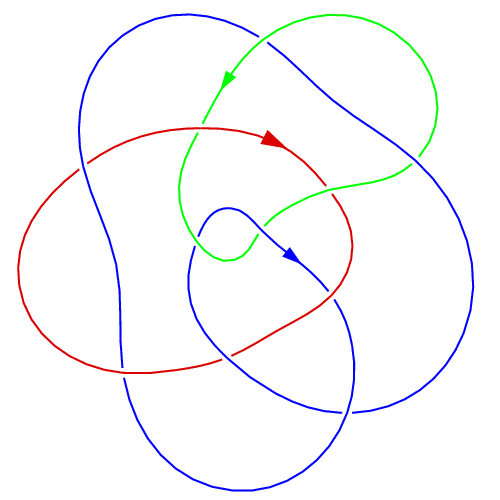
\includegraphics[width=\linewidth]{../data/link_mirror.png}
            \subcaption{lustro $mL$}
        \end{minipage}
        \begin{minipage}[b]{.32\linewidth}
            \centering
            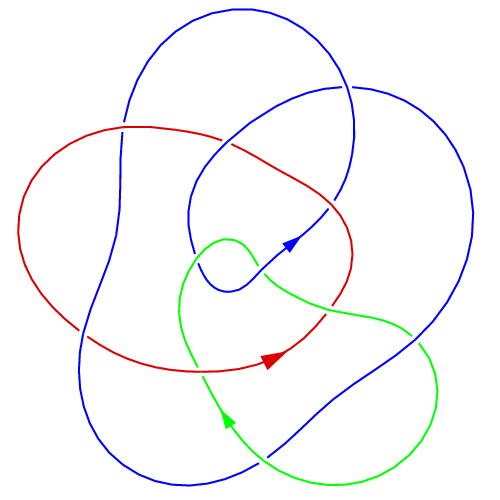
\includegraphics[width=\linewidth]{../data/link.png}
            \subcaption{przykładowy splot $L$}
        \end{minipage}
        \begin{minipage}[b]{.32\linewidth}
            \centering
            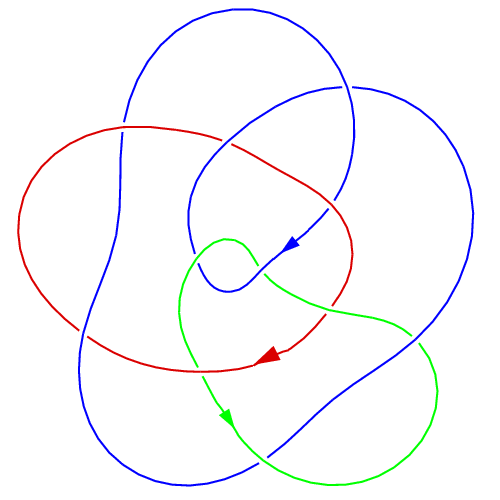
\includegraphics[width=\linewidth]{../data/link_reverse.png}
            \subcaption{rewers $rL$}
        \end{minipage}
    \end{figure}
\end{definition}

Na lewym obrazku odbiliśmy diagram względem poziomej prostej,
ale równie dobrze można po prostu zamienić każde nadskrzyżowanie na podskrzyżowanie.
Zauważmy, że wykonując powyższe operacje na węźle możemy otrzymać mniej niż czterech różne obiekty
($L$, $mL$, $rL$, $mrL$) -- na przykład trójlistnik jest własnym rewersem, ale nie lustrem.

\begin{definition}
    \index{węzeł!chiralny}
    \index{węzeł!odwracalny}
    \index{węzeł!zwierciadlany}
    Istnieje pięć typów symetrii węzłów:
    całkowicie chiralny albo skrętny (węzły $K$, $rK$, $mK$ są parami nierównoważne),
    odwracalny ($K \cong rK$),
    zwierciadlany ujemnie ($K \cong mrK$),
    zwierciadlany dodatnio ($K \cong mK$) oraz
    całkowicie zwierciadlany ($rK \cong K \cong mK$).
\end{definition}

Węzeł $9_{32}$ jest całkowicie skrętny.
Ósemka jest zwierciadlana, trójlistnik jest odwracalny,
zaś $8_{17}$ to najprostszy przykład węzła nieodwracalnego.
Ten ostatni fakt jest jednak daleki od oczywistego --
sześćdziesiąt lat temu nie było pewne,
czy węzły nieodwracalne w~ogóle istnieją.
W roku 1962 Ralph Fox wskazał kilku kandydatów do tego tytułu.
Hale Trotter odkrył rok później nieskończoną rodzinę nieodwracalnych precli (patrz \ref{def:pretzel}).
Obecnie wiadomo, że prawie wszystkie węzły są nieodwracalne (\cite[s.~46]{murasugi96}).
Wszystkie węzły torusowe są skrętne.

\begin{proposition}[Trotter, 1963] \label{trotter}
    Precel $(p, q, r)$, gdzie $p, q, r$ są parami różnymi liczbami całkowitymi, nie jest odwracalny.
\end{proposition}

\begin{proof}
    Praca \cite{trotter63} sprowadza w~elementarny sposób problem do pytania, czy pewna grupa posiada inwersję.
\end{proof}

Tait odnosił wrażenie, że zwierciadlane węzły mają parzysty indeks skrzyżowań,
ale Hoste (Thistlethwaite?) znalazł w~1998 kontrprzykład o~piętnastu skrzyżowaniach.
Jest on jedynym znanym nam dzisiaj.
Hipoteza Taita jest prawdziwa dla węzłów pierwszych, alternujących.

Poniższa tabela oparta jest (kolejno) o~ciągi
\href{https://oeis.org/A051766}{51766},
\href{https://oeis.org/A051769}{51769},
\href{https://oeis.org/A051768}{51768},
\href{https://oeis.org/A051767}{51767},
\href{https://oeis.org/A052400}{52400},
z bazy danych ``The On-Line Encyclopedia of Integer Sequences'' (OEIS).

\begin{table}[h]
    \centering
    \begin{tabular}{@{}*{20}l@{}} \toprule
        skrzyżowania & 3 & 4 & 5 & 6 & 7 & 8 & 9 & 10 & 11 & 12 & 13 & 14 \\ \midrule
        całkowicie skrętne & 0 & 0 & 0 & 0 & 0 & 0 & 2 & 27 & 187 & 1103 & 6919 & 37885 \\
        odwracalne & 1 & 0 & 2 & 2 & 7 & 16 & 47 & 125 & 365 & 1015 & 3069 & 8813 \\
        $-$ zwierciadlane & 0 & 0 & 0 & 0 & 0 & 1 & 0 & 6 & 0 & 40 & 0 & 227 \\
        $+$ zwierciadlane & 0 & 0 & 0 & 0 & 0 & 0 & 0 & 0 & 0 & 1 & 0 & 6 \\
        zwierciadlane & 0 & 1 & 0 & 1 & 0 & 4 & 0 & 7 & 0 & 17 & 0 & 41 \\
        \bottomrule
        \hline
    \end{tabular}
    \caption{Liczba węzłów o~poszczególnych typach symetrii}
    \label{tablica_wezlow}
\end{table}

Można wyróżnić jeszcze jeden rodzaj symetrii.

\begin{definition} \label{def_period}
    \index{węzeł!okresowy}
    Węzeł $K$ nazywamy $n$-okresowym, jeśli istnieje obrót $f \colon \R^3 \to \R^3$ o~kąt $2\pi/n$ wokół pewnej prostej $l$, rozłącznej z~węzłem, taki że $f(K) = K$.
\end{definition}

Trójlistnik jest 3-okresowy, węzeł $5_1$ 5-okresowy (widać to na standardowym diagramie) i~2-okresowy.
Tę drugą symetrię można dostrzec na diagramie realizującym indeks mostowy.

\begin{proposition}
    Zbiór wszystkich okresów jest niezmiennikiem węzłów.
\end{proposition}

Z~każdym węzłem okresowym związany jest inny, prostszy węzeł.
Niech $f$ będzie obrotem z definicji \ref{def_period}, zaś $p \colon \R^3 \to \R^3/f \simeq \R^3$ rzutem na przestrzeń ilorazową.
\index{węzeł!ilorazowy}
Wtedy $p(K)$ nazywamy \emph{węzłem ilorazowym}, zaś $K$ to jego $n$-krotne nakrycie.

Murasugi podał dwa warunki, które musi spełniać węzeł o~okresie $n = p^r$, gdzie $r$ jest liczbą pierwszą.
Do ich zrozumienia potrzebujemy prostej definicji.
Ustalmy półprostą, która nie jest styczna do węzła $K$, po czym zorientujmy ją oraz węzeł.
Indeksem zaczepienia $\lambda$ węzła $p(K)$ jest różnica między liczbą skrzyżowań dodatnich oraz ujemnych wzdłuż półprostej (bez znaku).

\begin{proposition}[warunek Murasugiego]
    \index{warunek Murasugiego}
    Niech $K$ będzie węzłem o~okresie $n = p^r$, gdzie $p$ jest liczbą pierwszą.
    Niech $J$ będzie jego węzłem ilorazowym, z~indeksem zaczepienia $\lambda$.
    Wtedy wielomian $\Delta_J$ jest dzielnikiem wielomianu $\Delta_K$ oraz istnieje pewna całkowita liczba $k$, taka że
    \[
        \Delta_K = \pm \Delta_J^n \left(1 + t + t^2 + \ldots + t^{\lambda - 1}\right)^{n-1} \mod p.
    \]
\end{proposition}

Dowód to, jak zwykle, mozolne operacje na macierzach.

% Koniec podsekcji Lustro i~rewers

\subsection{Suma niespójna i~suma spójna} % (fold)
\label{sub:knot_sum}
Suma spójna węzłów to szczególny przypadek sklejenia dwóch rozmaitości wzdłuż brzegu.

\begin{definition}
    \index{suma!niespójna}
    Niech $L_1, L_2$ będą splotami.
    Ich \textbf{sumą niespójną}, $L_1 \sqcup L_2$,
    jest teoriomnogościowa suma rozłączna splotów
    $L_1$ i~$L_2$ leżących po różnych stronach pewnej płaszczyzny.
\end{definition}

\begin{definition}
    \index{suma!spójna}
    Nacinając dwa zorientowane węzły w~dwóch bliskich punktach i
    ponownie zszywając je dwoma łukami nieprzecinającymi już
    istniejących otrzymujemy \textbf{sumę spójną}, $K_1 \shrap K_2$.
    \[
        \begin{tikzpicture}[baseline=-0.65ex,scale=0.1]
        \begin{knot}[clip width=5, flip crossing/.list={5}, ignore endpoint intersections=false,]
            \strand[thick] (-3.5, -3.5) [in=down, out=up] to (3.5, 3.5);
            \strand[thick] (3.5, 3.5) [in=right, out=up] to (-4.5, 10);
            \strand[thick] (-4.5, 10) [in=up, out=left] to (-10, 3.5);
            \strand[thick] (-10, 3.5) to (-10, -3.5);
            \strand[thick] (-10, -3.5) [in=left, out=down] to (-4.5, -10);
            \strand[thick] (-4.5, -10) [in=down, out=right] to (3.5, -3.5);
            \strand[thick] (3.5, -3.5) [in=down, out=up] to (-3.5, 3.5);
            \strand[thick] (-3.5, 3.5) [in=left, out=up] to (4.5, 10);
            \strand[thick] (4.5, 10) [in=up, out=right] to (10, 3.5);
            \strand[thick, -Latex] (10, 3.5) to (10, -3.5);
            \strand[thick] (10, -3.5) [in=right, out=down] to (4.5, -10);
            \strand[thick] (4.5, -10) [in=down, out=left] to (-3.5, -3.5);
            \node at (0, -15) {$K_1$};
        \end{knot}
        \end{tikzpicture}
        \shrap
        \begin{tikzpicture}[baseline=-0.65ex,scale=0.1]
        \begin{knot}[clip width=5, flip crossing/.list={6}, ignore endpoint intersections=false,]
            \strand[thick] (-3.5, -3.5) [in=down, out=up] to (3.5, 3.5);
            %\strand[thick] (3.5, 3.5) [in=right, out=up] to (-4.5, 10);
            %\strand[thick] (-4.5, 10) [in=up, out=left] to (-10, 3.5);
            \strand[thick] (-10, -3.5) [in=left, out=up] to (0, 6.5);
            \strand[thick, Latex-] (-10, -3.5) [in=left, out=down] to (-4.5, -10);
            \strand[thick] (-4.5, -10) [in=down, out=right] to (3.5, -3.5);
            \strand[thick] (3.5, -3.5) [in=down, out=up] to (-3.5, 3.5);
            %\strand[thick] (-3.5, 3.5) [in=left, out=up] to (4.5, 10);
            %\strand[thick] (4.5, 10) [in=up, out=right] to (10, 3.5);
            \strand[thick] (10, -3.5) [in=right, out=up] to (0, 6.5);
            \strand[thick] (10, -3.5) [in=right, out=down] to (4.5, -10);
            \strand[thick] (4.5, -10) [in=down, out=left] to (-3.5, -3.5);
            %
            \strand[thick] (-3.5, 3.5) [in=left, out=up] to (0, 10);
            \strand[thick] (3.5, 3.5) [in=right, out=up] to (0, 10);
            \node at (0, -15) {$K_2$};
        \end{knot}
        \end{tikzpicture}
        =
        \begin{tikzpicture}[baseline=-0.65ex,scale=0.1]
        \begin{knot}[clip width=5, flip crossing/.list={5, 22, 23}, ignore endpoint intersections=false,]
            \strand[thick] (-18.5, -3.5) [in=down, out=up] to (-11.5, 3.5);
            \strand[thick] (-11.5, 3.5) [in=right, out=up] to (-19.5, 10);
            \strand[thick] (-19.5, 10) [in=up, out=left] to (-25, 3.5);
            \strand[thick] (-25, 3.5) to (-25, -3.5);
            \strand[thick] (-25, -3.5) [in=left, out=down] to (-19.5, -10);
            \strand[thick] (-19.5, -10) [in=down, out=right] to (-11.5, -3.5);
            \strand[thick] (-11.5, -3.5) [in=down, out=up] to (-18.5, 3.5);
            \strand[thick] (-18.5, 3.5) [in=left, out=up] to (-10.5, 10);
            \strand[thick] (-10.5, 10) [in=left, out=right] to (-5, 2);
            \strand[thick, -Latex] (-5, 2) to (-5+6, 2);
            \strand[thick] (5, 2) to (-5+6, 2);
            \strand[thick] (3, -2) to [in=left, out=right] (10.5, -10);
            \strand[thick, -Latex] (3, -2) to (0, -2);
            \strand[thick] (-5, -2) to (0, -2);
            \strand[thick] (-5, -2) [in=right, out=left] to (-10.5, -10);
            \strand[thick] (-10.5, -10) [in=down, out=left] to (-18.5, -3.5);
            %%%
            \strand[thick] (11.5, -3.5) [in=down, out=up] to (18.5, 3.5);
            \strand[thick] (-10 +15, 2) [in=left, out=right] to (15, 6.5);
            \strand[thick] (10.5, -10) [in=down, out=right] to (18.5, -3.5);
            \strand[thick] (18.5, -3.5) [in=down, out=up] to (11.5, 3.5);
            \strand[thick] (25, -3.5) [in=right, out=up] to (15, 6.5);
            \strand[thick] (25, -3.5) [in=right, out=down] to (19.5, -10);
            \strand[thick] (19.5, -10) [in=down, out=left] to (11.5, -3.5);
            \strand[thick] (11.5, 3.5) [in=left, out=up] to (15, 10);
            \strand[thick] (18.5, 3.5) [in=right, out=up] to (15, 10);
            %%%
            \node at (0, -15) {$K_1 \shrap K_2$};
        \end{knot}
        \end{tikzpicture}
        \]
\end{definition}

Uogólnieniem tego działania oraz
(nieopisanej w~naszej pracy) operacji \emph{plumbing}
jest suma Murasugiego, dobrze wyjaśniona w~czwartym rozdziale \cite{kawauchi96}.

Ważna jest orientacja składników:
suma dwóch trójlistników może być,
w zależności od ich orientacji,
węzłem babskim\footnote{Nazewnictwo pochodzi od żeglarzy, nie matematyków. Z angielskiego \emph{granny knot}, \emph{square knot}.} lub prostym.
Fox pokazał w~1952 roku,
że dopełnienia tych dwóch węzłów nie są homeomorficzne.
Suma przeciwnie skręconych trójlistników jest plastrowa
(definicja \ref{def:slice_knot}),
natomiast tak samo skręconych -- nie.

\begin{proposition}
    Suma spójna jest dobrze określonym działaniem.
\end{proposition}

Suma spójna nie jest dobrze określona dla splotów:
nie istnieje kanoniczny wybór, które składowe łączyć ze sobą.

\begin{proof}
    Niech dane będą węzły $K_1$ oraz $K_2$
    oraz dwa różne łuki $\gamma_1$, $\gamma_2$,
    których można użyć do konstrukcji sumy spójnej.
    Skurczmy $K_1$, przeciągnijmy najpierw przez łuk $\gamma_1$, a~następnie wzdłuż węzła $K_2$.
    Teraz wystarczy odwrócić ten proces z~$\gamma_2$ w~miejscu $\gamma_1$.
\end{proof}

\begin{proposition}
    Suma spójna zorientowanych węzłów posiada następujące własności:
    \begin{enumerate}[leftmargin=*]
    \itemsep0em
        \item jest łączna:
        $(K_1 \shrap K_2) \shrap K_3 \simeq K_1 \shrap (K_2 \shrap K_3)$,
        \item jest przemienna:
        $K_1 \shrap K_2 \simeq K_2 \shrap K_1$,
        \item posiada element neutralny:
        $K_1 \shrap \LittleUnknot \simeq \LittleUnknot \shrap K_1 \simeq K_1$.
    \end{enumerate}
\end{proposition}

Prosty dowód tego faktu pozostawiamy Czytelnikowi.
Pokażemy za to, iż węzły z~sumą spójną nie tworzą grupy -- brakuje elementów przeciwnych.

\begin{proposition}
    Jeśli $K \shrap L = \Unknot$, to $K = L = \Unknot$.
\end{proposition}

\begin{proof}[Niedowód]
    Technika ta zwana jest szwindlem Mazura.
    Załóżmy, że $K \shrap L = \Unknot$ i~dopuśćmy wyjątkowo węzły dzikie.
    Skonstruujmy sumę $K \shrap L \shrap K \shrap \ldots$,
    przy czym kolejne składniki powinny zmniejszać się,
    aby ich suma nadal była węzłem.
    Wtedy
    \begin{align*}
        K & \simeq K \shrap [(L \shrap K) \shrap (L \shrap K) \ldots] \\
         & \simeq (K \shrap L) \shrap (K \shrap L) \shrap \ldots
         \simeq \Unknot \shrap \Unknot \shrap \ldots
         \simeq \Unknot.
    \end{align*}
    Analogicznie pokazujemy, że $L \simeq \Unknot$.
\end{proof}

Później poznamy prawdziwy, oparty na topologii algebraicznej, dowód.
Połączymy fakty \ref{genus_one} oraz \ref{genus_sum}.

Półgrupę węzłów z~operacją sumy spójnej można ulepszyć do grupy na dwa sposoby:
albo poprzez zmianę działania, w~jakie jest wyposażona,
albo osłabiając definicję węzłów równoważnych.
Drugi pomysł jest dużo lepszy niż pierwszy.
Na początku lat pięćdziesiątych J. Milnor wprowadził do matematyki pojęcie zgodności
(z angielskiego \emph{concordance}), które zastąpiło zwykłą równoważność.
Element neutralny nowej grupy to węzły plastrowe, ich opis leży w~sekcji \ref{sec:slice}.
Zagadnienia te zakorzenione są w~czterowymiarowej topologii.

% Koniec podsekcji Suma niespójna i~suma spójna

% Koniec sekcji Operacje na węzłach

\section{Węzły pierwsze}
\label{sec:prime_knots}
Istnieje węzłowy odpowiednik liczb pierwszych.
Jest on ściśle związany z podaną wyżej operacją sumy spójnej.
Do jego dostatecznie dobrego zrozumienia wymagana jest znajomość powierzchni Seiferta (opisanych w sekcji \ref{sec:genus}).

\begin{definition} \label{primeknot}
    Nietrywialny węzeł nazywamy \textbf{pierwszym},
    kiedy nie można przedstawić go jako sumy spójnej $K_1 \shrap K_2$
    dwóch nietrywialnych węzłów $K_1, K_2$ (nie jest złożony).
\end{definition}

Okazuje się, że jeśli alternujący \todo{definicja splotów alternujących} splot nie jest pierwszy,
to każdy jego alternujący diagram jest złożony.
Jako pierwszy fakt ten został wykazany przez Menasco w \cite{menasco84}.
Dowód opiera się na multiplikatywności wielomianu BLM/Ho (opisuje go definicja \ref{def:blm_ho}).

Czy węzłów pierwszych jest nieskończenie wiele?
Tak (patrz fakt \ref{infty_primes}), potrafimy nawet oszacować ich liczbę.
W roku 1987 C. Ernst, D. Sumners w oparciu o wyniki Thistlethwaite'a, Kauffmana, oraz Murasugiego dotyczące węzłów alternujących pokazali w \cite{ernst87},
że różnych węzłów pierwszych o $n$ skrzyżowaniach jest co najmniej $\frac 1 3 (2^{n- 2} - 1)$ dla $n \ge 4$,
przy czym węzły lustrzane traktowane są jako różne.
Welsh znalazł ograniczenie
\[
    \limsup_{n \to \infty} \sqrt[n]{N(n)} \le 13.5,
\]
gdzie $N(n)$ jest ilością pierwszych węzłów o $n$ skrzyżowaniach.

Czy niewęzeł nie daje się zapisać jako suma dwóch innych węzłów?
Byłoby to skrajnie niepożądane, gdyż każdy węzeł jest naturalnie spójną sumą siebie oraz niewęzła.
Na szczęście przy pomocy powierzchni Seiferta można pokazać, że tak się nie dzieje (jest to wniosek \ref{no_inverses}).
Prawdziwe jest dużo mocniejsze stwierdzenie,
którego nie udowodnimy ze względu na niedostatecznie rozwinięty aparat matematyczny.
Należy o nim myśleć jak o analogonie zasadniczego twierdzenia arytmetyki.

\begin{theorem}[Schubert, 1949]
    Każdy różny od niewęzła węzeł rozkłada się jednoznacznie na węzły pierwsze
    (jeśli tylko pominąć kolejność składników).
\end{theorem}

Pomimo to uda się nam pokazać samo istnienie rozkładu, jest to fakt \ref{genus_sum}.
% koniec sekcji Węzły pierwsze

\section{Niezmienniki liczbowe}
Jak wspomnieliśmy na początku rozdziału, sprawdzenie,
czy dwa diagramy przedstawiają sploty równoważne,
jest uciążliwym i czasochłonnym zadaniem.
Aby je uprościć, podamy opis kilku prostych niezmienników o całkowitych wartościach.
Zachodzą implikacje:
sploty równoważne $\Rightarrow$ ta sama wartość niezmiennika
oraz różne wartości niezmiennika $\Rightarrow$ różne sploty.

\subsection{Indeks skrzyżowaniowy} % (fold)
\label{sub:crossing_number}
Z angielskiego \emph{crossing number}.

\begin{definition}
    Indeks skrzyżowaniowy $\operatorname{cr}(L)$ splotu $L$ to
    minimalna liczba skrzyżowań widocznych na diagramie,
    który przedstawia splot $L$.
\end{definition}

Wciąż nie jest wiadome, czy indeks skrzyżowaniowy jest addytywny względem sumy spójnej.
Potrafimy to jednak udowodnić dla niektórych węzłów: alternujących, adekwatnych czy torusowych.
Lackenby w pracy \cite{lackenby09} pokazał, że dla pewnej stałej $N > 1$ zachodzi
\[
    \operatorname{cr} L_1 + \operatorname{cr} L_2 \le N \cdot \operatorname{cr} (L_1 \# L_2).
\]
Jego podejście (przez powierzchnie normalne) nie jest w stanie poprawić stałej do $N = 1$.

% Koniec podsekcji Indeks skrzyżowaniowy

\subsection{Liczba gordyjska} % (fold)
\label{sub:unknotting_number}
Z angielskiego \emph{unknotting number}.

\begin{definition}
    Liczba gordyjska $\operatorname{u}(K)$ węzła $K$ to minimalna liczba skrzyżowań,
    które trzeba odwrócić na pewnym jego diagramie, by dostać niewęzeł.
    Liczba $u$ nie musi być osiągana przez diagram o minimalnej liczbie skrzyżowań.
\end{definition}

Dotychczas wyznaczono liczbę gordyjską dla prawie wszystkich węzłów pierwszych o co najwyżej dziesięciu skrzyżowaniach,
Cha i Livingston podają następującą listę wyjątków: 
$10_{11}$, $10_{47}$, $10_{51}$, $10_{54}$, $10_{61}$, $10_{76}$, $10_{77}$, $10_{79}$, $10_{100}$ (stan na rok 2008).
S. Bleiler odkrył w \cite{bleiler84} fascynujący przykład wymiernego węzła $2$-gordyjskiego,
czego świadkiem nie może być diagram o minimalnej liczbie skrzyżowań
(ponieważ, co jeszcze bardziej fascynujące, węzeł ten posiada tylko jeden diagram o dziesięciu skrzyżowaniach z trzema do odwrócenia).
Koduje go liczba $29/6$, w tabeli węzłów figuruje jako $10_8$.
Stoimenow w \cite{stoimenow01} pokazuje, że jeden węzeł może mieć kilka diagramów minimalnych,
z których tylko niektóre są świadkiem $1$-gordyjskości (są to między innymi $14_{36750}$ oraz $14_{36760}$.)

Jeśli odwrócenie pewnych skrzyżowań daje niewęzeł, to odwrócenie pozostałych także.
To daje proste, choć niezbyt pomocne oszacowanie liczby gordyjskiej: $2 \operatorname{u} (K) \le \operatorname{cr} (K)$. 
Borodzik oraz Friedl podali niedawno całkiem mocne ograniczenia na liczbę gordyjską w pracach \cite{borodzik14} i \cite{borodzik15} opierając się o parowanie Blanchfielda
(poprawiając ograniczenia z sygnatury Levine'a-Tristrama, indeksu Nakanishiego oraz przeszkodą Lickorisha).
Dwadzieścia pięć węzłów o co najwyżej dwunastu skrzyżowaniach ma liczbę gordyjską równą co najmniej trzy, co trudno pokazać innymi metodami.

Dla każdego nietrywialnego splotu istnieje diagram wymagający odwrócenia  dowolnie wielu skrzyżowań (dowód zawiera praca \cite{taniyama09} Taniyamy).
Pokazany jest tam jeszcze jeden godny uwagi fakt.
Jeśli liczba gordyjska diagramu $D$ wynosi $\frac 12 (c(D) - 1)$,
co jest maksymalną możliwą wartością zgodnie z naszym prostym ograniczeniem,
to węzeł jest $(2,p)$-torusowy albo wygląda jak diagram niewęzła po pierwszym ruchu Reidemeistera.

% Liczba gordyjska nietrywialnego węzła skręconego (definicja \ref{twist_knots}) to jeden, wystarczy bowiem rozwiązać jego splecione końce.
Patrz także stwierdzenie \ref{torus_unknotting}.

Od początku teorii węzłów podejrzewano, że liczba gordyjska jest addytywna, to znaczy $u(K \shrap J) = u(K) + u(J)$.
Z tej nieudowodnionej do dzisiaj hipotezy można wyciągnąć wniosek,
że jeśli do rozwiązania węzła wystarcza odwrócenie skrzyżowania, to jest pierwszy.
Podejrzewał to H. Wendt w 1937 roku,
kiedy policzył liczbę gordyjską węzła babskiego używając homologii rozgałęzionego nakrycia cyklicznego.

\begin{proposition}
    Węzły $1$-gordyjskie są pierwsze.
\end{proposition}

\begin{proof}[Niedowód]
    W pracy \cite{scharleman85} z 1985 roku M. Scharleman podał dość zawiłe uzasadnienie, w które zamieszane były grafy planarne.
\end{proof}

W pracy \cite{shimizu14} Ayaka Shimizu pokazuje przykład innej operacji rozwiązującej węzły, ale nie sploty:
zmianę skrzyżowań wokół obszaru na diagramie.

Przestrzeń gordyjska
(wszystkich węzłów wyposażona w metrykę pochodzącą od liczby gordyjskiej)
bywa sprzeczna z intuicją.
W pracy ,,Braids and signatures'' J. Gambaudo, E. Ghys (twierdzenie C) pokazali,
że przestrzeń węzłów zawiera prawie idalną kopię przestrzeni euklidesowej dowolnego wymiaru.
Dokładniej:

\begin{proposition}
    Dla każdej liczby całkowitej $d \ge 1$ istnieje funkcja $\xi: \Z^d \to \mathcal{K}$, która dla pewnych stałych $A, B, C \ge 0$ i pewnej normy $\|\cdot\|$ spełnia podwójną nierówność
    \[
        A\|x-y\|  - B \le d(\xi(x), \xi(y)) \le C\|x-y\|.
    \]
\end{proposition}

% Koniec podsekcji Liczba gordyjska

\subsection{Liczba mostowa} % (fold)
\label{sub:bridge_index}
Z angielskiego \emph{bridge number}.
Wprowadzona w 1954 przez Schuberta.
\begin{definition}
    Liczba mostowa $\operatorname{br}(K)$ to minimalna liczba mostów:
    długich łuków, które biegną przez nadskrzyżowania.
\end{definition}

Można pokazać, że $n$-mostowe węzły rozkładają się na sumę dwóch trywialnych $n$-supłów.

\begin{proposition}
    Niech $K_1, K_2$ będą węzłami.
    Wtedy $\operatorname{br} (K_1) + \operatorname{br}(K_2) = \operatorname{br}(K_1 \# K_2) + 1$.
\end{proposition}

\begin{proof}
    Schultens w artykule \cite{schultens03} dowodzi (przy użyciu foliacji na brzegu węzła towarzysza w satelitarnym) jeszcze raz tego, co pokazał Schubert w \cite{schubert54}.
    Z tego względu nie możemy tutaj opowiedzieć o szczegółach technicznych dowodu.
\end{proof}

Tylko jeden węzeł jest jednomostowy, to niewęzęł.
Kolejne w hierarchi skomplikowania, czyli dwumostowe,
to domknięcia wymiernych supłów, patrz fakt \ref{two_bridge_tangle}.
Węzły trójmostowe pozostają nie do końca zbadane.

\todo[inline]{Hipoteza mówi, że $c \ge 3 br - 3$, z równością dla inewęzła i sum trójlistników.}

% Koniec podsekcji Liczba mostowa

\subsection{Liczba warkoczowa} % (fold)
\label{sub:braid_number}
Z angielskiego \emph{braid number}.
Do jej określenia potrzebna jest definicja \ref{braid_def}.

\begin{definition}
    Liczba warkoczowa to minimalna liczba pasm, na których można zbudować warkocz, którego domknięciem jest wyjściowy węzeł.
\end{definition}

\begin{proposition}
    Węzeł o $n$ skrzyżowaniach można zapleść na $n - 1$ pasmach.
\end{proposition}

Indeks warkoczowy zależy od orientacji ogniw i trudno się go wyznacza w ogólnym przypadku.
Poniższy dowód zakłada znajomość warkoczy (rozdział piąty).

\begin{proposition}
    Indeksem warkoczowym węzła torusowego $K(q, r)$, $rq \neq 0$, jest $\min\{|q|, |r|\}$.
\end{proposition}

\begin{proof}
Niech $K$ będzie węzłem torusowym typu $(q,r)$ z minimalnym przedstawieniem jako warkocz $\beta$.
Z konstrukcji domknięcia (czyli dołączenia rozłącznych półokręgów) wynika, 
że diagram $K$ ma dokładnie $b(K)$ lokalnych maksimów.
Definicja indeksu mostowego orzeka, iż $br(K) \le b(K)$.
Bez straty ogólności niech $q > r > 0$.
Skoro węzeł $K$ powstaje z $r$-warkocza $(\sigma_{r-1} \ldots \sigma_2\sigma_1)^q$, 
indeks $b(K)$ nie przekracza $r = br(K)$.

Skorzystaliśmy z faktu \ref{torus_bridge}.
\end{proof} 

% Koniec podsekcji Liczba warkoczowa

\subsection{Indeks zaczepienia} % (fold)
\label{sub:linking_number}
\begin{definition} \label{sign_def}
    Na diagramie zorientowanego splotu, każdemu skrzyżowaniu przypisujemy \textbf{znak} równy $\pm 1$.
    Skrzyżowania dodatnie nazywamy praworęcznymi, ujemne zaś: leworęcznymi.
    \[
        \sign \Bigl(\,\,\begin{tikzpicture}[baseline=-0.65ex,scale=0.07]
        \begin{knot}[clip width=5]
        \strand[semithick,-Latex] (-5,-5) -- (5,5);
        \strand[semithick,Latex-] (-5,5) -- (5,-5);
        \end{knot}\end{tikzpicture}\,\,\Bigr) = +1 \quad
        \sign \Bigl(\,\,\begin{tikzpicture}[baseline=-0.65ex,scale=0.07]
        \begin{knot}[clip width=5, flip crossing/.list={1}]
        \strand[semithick,-Latex] (-5,-5) -- (5,5);
        \strand[semithick,Latex-] (-5,5) -- (5,-5);
        \end{knot}\end{tikzpicture}\,\,\Bigr) = -1
    \]
    \textbf{Indeks zaczepienia} splotu zorientowanego $L$ o diagramie $D$ to $\frac 12 \sum_c \sign (c)$,
    gdzie $c$ przebiega każde skrzyżowanie, przy którym spotykają się \emph{różne} składowe.
    Oznaczenie: $\operatorname{lk}(L)$.
\end{definition}

Zauważmy, że indeks zaczepienia splotu Hopfa wynosi $1$, natomiast splotu Whiteheada $0$.
Są więc istotnie różne.

\begin{proposition}
    Indeks zaczepienia jest dobrze określonym niezmiennikiem zorientowanych węzłów.
\end{proposition}

\begin{proof}
    Sprawdźmy wpływ ruchów Reidemeistera na wartość
    $\operatorname{lk}(L)$:

    \[
        \fbox{
        \begin{tikzpicture}[baseline=-0.65ex,scale=0.07]
        \begin{knot}[clip width=5]
        \strand[semithick] (-10,10) .. controls (-10,2) and (-10,2) .. (-6,-2);
        \strand[semithick] (-10,-10) .. controls (-10,-2) and (-10,-1) .. (-9,0);
        \strand[semithick] (-7,1) -- (-6,2);
        \strand[semithick] (-6,2) .. controls (2,9) and (2,-9) .. (-6,-2);
        \end{knot}
        \end{tikzpicture}
        $\stackrel{R_1}{\cong} \,\,$
        \begin{tikzpicture}[baseline=-0.65ex,scale=0.07]
        \begin{knot}[clip width=5]
        \strand[semithick] (0,10) -- (0,-10);
        \end{knot}
        \end{tikzpicture}}
        %%%
        \quad \fbox{
        \begin{tikzpicture}[baseline=-0.65ex,scale=0.07]
        \begin{knot}[clip width=5]
        \strand[semithick] (4,-10) .. controls (4,-4) and (-4,-4) .. (-4,0);
        \strand[semithick] (4,10) .. controls (4, 4) and (-4, 4) .. (-4,0);
        \strand[semithick] (-4,-10) .. controls (-4,-4) and (4,-4) .. (4,0);
        \strand[semithick] (-4,10) .. controls (-4, 4) and (4,4) .. (4,0);
        \node[blue] at (-4,4)[left] {$a$};
        \node[blue] at (-4,-4)[left] {$-a$};
        \end{knot}
        \end{tikzpicture}
        $\stackrel{R_2}{\cong} \,\,$
        \begin{tikzpicture}[baseline=-0.65ex,scale=0.07]
        \begin{knot}[clip width=5]
        \strand[semithick] (4,-10) .. controls (4,-4) and (1,-4) .. (1,0);
        \strand[semithick] (4,10) .. controls (4, 4) and (1, 4) .. (1,0);
        \strand[semithick] (-4,-10) .. controls (-4,-4) and (-1,-4) .. (-1,0);
        \strand[semithick] (-4,10) .. controls (-4, 4) and (-1,4) .. (-1,0);
        \end{knot}
        \end{tikzpicture}}
        %%%
        \quad \fbox{
        \begin{tikzpicture}[baseline=-0.65ex,scale=0.07]
        \begin{knot}[clip width=5, flip crossing/.list={1,2,3}]
        \strand[semithick] (-10,-10) -- (10,10);
        \strand[semithick] (-10,10) -- (10,-10);
        \strand[semithick] (-10,-2) .. controls (-4, -2) and (-4,8) .. (0,8);
        \strand[semithick] (10,-2) .. controls (4, -2) and (4,8) .. (0,8);
        \node[blue] at (-6,4)[left] {$a$};
        \node[blue] at (6,4)[right] {$b$};
        \node[blue] at (0,-2)[below] {$c$};
        \end{knot}
        \end{tikzpicture}
        $\stackrel{R_3}{\cong} \,\,$
        \begin{tikzpicture}[baseline=-0.65ex,scale=0.07]
        \begin{knot}[clip width=5, flip crossing/.list={1,2,3}]
        \strand[semithick] (-10,-10) -- (10,10);
        \strand[semithick] (-10,10) -- (10,-10);
        \strand[semithick] (-10,2) .. controls (-4, 2) and (-4,-8) .. (0,-8);
        \strand[semithick] (10,2) .. controls (4, 2) and (4,-8) .. (0,-8);
        \node[blue] at (-6,-4)[left] {$a$};
        \node[blue] at (6,-4)[right] {$b$};
        \node[blue] at (0,2)[above] {$c$};
        \end{knot}
        \end{tikzpicture}}
    \]
    Na mocy twierdzenia Reidemeistera dowód został zakończony.
\end{proof}

\todo[inline]{Linking number jest zawsze całkowita (tw. Jordana)}

% Koniec podsekcji Indeks zaczepienia

\subsection{Sygnatura} % (fold)
\label{sub:signature}
Sygnatura pojawia się w fakcie \ref{slice_signature}.

\begin{definition}
    Sygnatura to niezmiennik topologiczny zadany (kłębiastą) relacją rekurencyjną:
    \begin{itemize}[leftmargin=*]
    \itemsep0em
        \item $\sigma (\MalyNieWezel) = 0$,
        \item $\sigma (K_+) - \sigma (K_-) \in \{0, 2\}$,
        \item $4 \mid \sigma (K)$ wtedy i tylko wtedy, gdy $\nabla(2i) > 0$ (wielomian Conwaya).
    \end{itemize}
\end{definition}

Sygnatura pozwala uzyskać proste oszacowanie liczby gordyjskiej od dołu:

\begin{proposition}
    Mamy $2 u(K) \ge |\sigma(K)|$.
\end{proposition}

Nie istnieje bezpośredni związek między sygnaturą i liczbą mostową.
Węzeł torusowy $T_{2,n}$ jest dwumostowy, jego sygnatura wynosi $n - 1$.
Suma spójna węzłów prostych ma zerową sygnaturę i nieograniczoną liczbę mostową.

% Koniec podsekcji Sygnatura

% Koniec sekcji Niezmienniki liczbowe


\chapter{Niezmienniki kolorowe}

\chapter{Niezmienniki wielomianowe}

\chapter{Topologia algebraiczna}

\chapter{Wybrane rodziny węzłów}

\chapter{Tablice węzłów pierwszych}
\section{Wartości niezmienników}
\label{sec:table_of_invariants}
Tabela przedstawia węzły pierwsze o~co najwyżej dziesięciu skrzyżowaniach oraz wartości ich niezmienników (całkowitoliczbowych lub wielomianowych).
Zgodnie z~oznaczeniami przyjętymi w reszcie książki, $\operatorname{u}, \operatorname{b}, \operatorname{br}$ to kolejno liczba gordyjska, warkoczowa i~mostowa.
Zapis $2..3$ mówi, że dokładna wartość nie jest znana i leży w przedziale $[2,3]$.
Jeśli liczba mostowa wynosi dokładnie $2$, zamiast niej podajemy nieskracalny ułamek $p/q$, który koduje węzeł.
Dalej, $\det$ jest wyznacznikiem, $\sigma$ sygnaturą, Arf -- oczywiście niezmiennikiem Arfa.
Wielomian Conwaya $\nabla(z)$ dla oszczędności miejsca podajemy jako ciąg współczynników, na przykład $1-1$ jest skrótem od $1-z^2$.

Dane zawarte w~tej tabeli pochodzą ze strony \url{http://www.indiana.edu/~knotinfo/}.
Jej autorzy, Chuck Livingston z~uniwersytetu Indiany  oraz Jae Choon Cha (z koreańskiego Pohangu) prezentują tam wiele innych niezmienników.

\renewcommand*{\arraystretch}{1.4}
\footnotesize
\begin{longtable}{lccccccllc}
\hline
nazwa & u~& b & br & $\det$ & sygn. & Arf & $\nabla(z)$ & sym. & alt. \\ \hline
\endhead % all the lines above this will be repeated on every page
$3_{1}$     &  $1$     &  $2$  &  $3/1$    &  $3$    &  $-2$  &  $1$  &  $1+1$          &  odwracalny  &  tak  \\
$4_{1}$     &  $1$     &  $3$  &  $5/2$    &  $5$    &  $0$   &  $1$  &  $1-1$          &  całkowicie  &  tak  \\
$5_{1}$     &  $2$     &  $2$  &  $5/1$    &  $5$    &  $-4$  &  $1$  &  $1+3+1$        &  odwracalny  &  tak  \\
$5_{2}$     &  $1$     &  $3$  &  $7/3$    &  $7$    &  $-2$  &  $0$  &  $1+2$          &  odwracalny  &  tak  \\
$6_{1}$     &  $1$     &  $4$  &  $9/7$    &  $9$    &  $0$   &  $0$  &  $1-2$          &  odwracalny  &  tak  \\
$6_{2}$     &  $1$     &  $3$  &  $11/4$   &  $11$   &  $-2$  &  $1$  &  $1-1-1$        &  odwracalny  &  tak  \\
$6_{3}$     &  $1$     &  $3$  &  $13/5$   &  $13$   &  $0$   &  $1$  &  $1+1+1$        &  całkowicie  &  tak  \\
$7_{1}$     &  $3$     &  $2$  &  $7/1$    &  $7$    &  $-6$  &  $0$  &  $1+6+5+1$      &  odwracalny  &  tak  \\
$7_{2}$     &  $1$     &  $4$  &  $11/5$   &  $11$   &  $-2$  &  $1$  &  $1+3$          &  odwracalny  &  tak  \\
$7_{3}$     &  $2$     &  $3$  &  $13/9$   &  $13$   &  $-4$  &  $1$  &  $1+5+2$        &  odwracalny  &  tak  \\
$7_{4}$     &  $2$     &  $4$  &  $15/11$  &  $15$   &  $-2$  &  $0$  &  $1+4$          &  odwracalny  &  tak  \\
$7_{5}$     &  $2$     &  $3$  &  $17/7$   &  $17$   &  $-4$  &  $0$  &  $1+4+2$        &  odwracalny  &  tak  \\
$7_{6}$     &  $1$     &  $4$  &  $19/7$   &  $19$   &  $-2$  &  $1$  &  $1+1-1$        &  odwracalny  &  tak  \\
$7_{7}$     &  $1$     &  $4$  &  $21/8$   &  $21$   &  $0$   &  $1$  &  $1-1+1$        &  odwracalny  &  tak  \\
$8_{1}$     &  $1$     &  $5$  &  $13/11$  &  $13$   &  $0$   &  $1$  &  $1-3$          &  odwracalny  &  tak  \\
$8_{2}$     &  $2$     &  $3$  &  $17/6$   &  $17$   &  $-4$  &  $0$  &  $1+0-3-1$      &  odwracalny  &  tak  \\
$8_{3}$     &  $2$     &  $5$  &  $17/4$   &  $17$   &  $0$   &  $0$  &  $1-4$          &  całkowicie  &  tak  \\
$8_{4}$     &  $2$     &  $4$  &  $19/14$  &  $19$   &  $2$   &  $1$  &  $1-3-2$        &  odwracalny  &  tak  \\
$8_{5}$     &  $2$     &  $3$  &  $3$      &  $21$   &  $-4$  &  $1$  &  $1-1-3-1$      &  odwracalny  &  tak  \\
$8_{6}$     &  $2$     &  $4$  &  $23/10$  &  $23$   &  $-2$  &  $0$  &  $1-2-2$        &  odwracalny  &  tak  \\
$8_{7}$     &  $1$     &  $3$  &  $23/9$   &  $23$   &  $2$   &  $0$  &  $1+2+3+1$      &  odwracalny  &  tak  \\
$8_{8}$     &  $2$     &  $4$  &  $25/9$   &  $25$   &  $0$   &  $0$  &  $1+2+2$        &  odwracalny  &  tak  \\
$8_{9}$     &  $1$     &  $3$  &  $25/7$   &  $25$   &  $0$   &  $0$  &  $1-2-3-1$      &  całkowicie  &  tak  \\
$8_{10}$    &  $2$     &  $3$  &  $3$      &  $27$   &  $2$   &  $1$  &  $1+3+3+1$      &  odwracalny  &  tak  \\
$8_{11}$    &  $1$     &  $4$  &  $27/10$  &  $27$   &  $-2$  &  $1$  &  $1-1-2$        &  odwracalny  &  tak  \\
$8_{12}$    &  $2$     &  $5$  &  $29/12$  &  $29$   &  $0$   &  $1$  &  $1-3+1$        &  całkowicie  &  tak  \\
$8_{13}$    &  $1$     &  $4$  &  $29/11$  &  $29$   &  $0$   &  $1$  &  $1+1+2$        &  odwracalny  &  tak  \\
$8_{14}$    &  $1$     &  $4$  &  $31/12$  &  $31$   &  $-2$  &  $0$  &  $1+0-2$        &  odwracalny  &  tak  \\
$8_{15}$    &  $2$     &  $4$  &  $3$      &  $33$   &  $-4$  &  $0$  &  $1+4+3$        &  odwracalny  &  tak  \\
$8_{16}$    &  $2$     &  $3$  &  $3$      &  $35$   &  $2$   &  $1$  &  $1+1+2+1$      &  odwracalny  &  tak  \\
$8_{17}$    &  $1$     &  $3$  &  $3$      &  $37$   &  $0$   &  $1$  &  $1-1-2-1$      &  ujemny      &  tak  \\
$8_{18}$    &  $2$     &  $3$  &  $3$      &  $45$   &  $0$   &  $1$  &  $1+1-1-1$      &  całkowicie  &  tak  \\
$8_{19}$    &  $3$     &  $3$  &  $3$      &  $3$    &  $-6$  &  $1$  &  $1+5+5+1$      &  odwracalny  &  nie  \\
$8_{20}$    &  $1$     &  $3$  &  $3$      &  $9$    &  $0$   &  $0$  &  $1+2+1$        &  odwracalny  &  nie  \\
$8_{21}$    &  $1$     &  $3$  &  $3$      &  $15$   &  $-2$  &  $0$  &  $1+0-1$        &  odwracalny  &  nie  \\
$9_{1}$     &  $4$     &  $2$  &  $9/1$    &  $9$    &  $-8$  &  $0$  &  $1+10+15+7+1$  &  odwracalny  &  tak  \\
$9_{2}$     &  $1$     &  $5$  &  $15/7$   &  $15$   &  $-2$  &  $0$  &  $1+4$          &  odwracalny  &  tak  \\
$9_{3}$     &  $3$     &  $3$  &  $19/13$  &  $19$   &  $-6$  &  $1$  &  $1+9+9+2$      &  odwracalny  &  tak  \\
$9_{4}$     &  $2$     &  $4$  &  $21/5$   &  $21$   &  $-4$  &  $1$  &  $1+7+3$        &  odwracalny  &  tak  \\
$9_{5}$     &  $2$     &  $5$  &  $23/17$  &  $23$   &  $-2$  &  $0$  &  $1+6$          &  odwracalny  &  tak  \\
$9_{6}$     &  $3$     &  $3$  &  $27/5$   &  $27$   &  $-6$  &  $1$  &  $1+7+8+2$      &  odwracalny  &  tak  \\
$9_{7}$     &  $2$     &  $4$  &  $29/13$  &  $29$   &  $-4$  &  $1$  &  $1+5+3$        &  odwracalny  &  tak  \\
$9_{8}$     &  $2$     &  $5$  &  $31/11$  &  $31$   &  $-2$  &  $0$  &  $1+0-2$        &  odwracalny  &  tak  \\
$9_{9}$     &  $3$     &  $3$  &  $31/9$   &  $31$   &  $-6$  &  $0$  &  $1+8+8+2$      &  odwracalny  &  tak  \\
$9_{10}$    &  $3$     &  $4$  &  $33/23$  &  $33$   &  $-4$  &  $0$  &  $1+8+4$        &  odwracalny  &  tak  \\
$9_{11}$    &  $2$     &  $4$  &  $33/14$  &  $33$   &  $4$   &  $0$  &  $1+4-1-1$      &  odwracalny  &  tak  \\
$9_{12}$    &  $1$     &  $5$  &  $35/13$  &  $35$   &  $-2$  &  $1$  &  $1+1-2$        &  odwracalny  &  tak  \\
$9_{13}$    &  $3$     &  $4$  &  $37/27$  &  $37$   &  $-4$  &  $1$  &  $1+7+4$        &  odwracalny  &  tak  \\
$9_{14}$    &  $1$     &  $5$  &  $37/14$  &  $37$   &  $0$   &  $1$  &  $1-1+2$        &  odwracalny  &  tak  \\
$9_{15}$    &  $2$     &  $5$  &  $39/16$  &  $39$   &  $2$   &  $0$  &  $1+2-2$        &  odwracalny  &  tak  \\
$9_{16}$    &  $3$     &  $3$  &  $3$      &  $39$   &  $-6$  &  $0$  &  $1+6+7+2$      &  odwracalny  &  tak  \\
$9_{17}$    &  $2$     &  $4$  &  $39/14$  &  $39$   &  $-2$  &  $0$  &  $1-2+1+1$      &  odwracalny  &  tak  \\
$9_{18}$    &  $2$     &  $4$  &  $41/17$  &  $41$   &  $-4$  &  $0$  &  $1+6+4$        &  odwracalny  &  tak  \\
$9_{19}$    &  $1$     &  $5$  &  $41/16$  &  $41$   &  $0$   &  $0$  &  $1-2+2$        &  odwracalny  &  tak  \\
$9_{20}$    &  $2$     &  $4$  &  $41/15$  &  $41$   &  $-4$  &  $0$  &  $1+2-1-1$      &  odwracalny  &  tak  \\
$9_{21}$    &  $1$     &  $5$  &  $43/18$  &  $43$   &  $2$   &  $1$  &  $1+3-2$        &  odwracalny  &  tak  \\
$9_{22}$    &  $1$     &  $4$  &  $3$      &  $43$   &  $-2$  &  $1$  &  $1-1+1+1$      &  odwracalny  &  tak  \\
$9_{23}$    &  $2$     &  $4$  &  $45/19$  &  $45$   &  $-4$  &  $1$  &  $1+5+4$        &  odwracalny  &  tak  \\
$9_{24}$    &  $1$     &  $4$  &  $3$      &  $45$   &  $0$   &  $1$  &  $1+1-1-1$      &  odwracalny  &  tak  \\
$9_{25}$    &  $2$     &  $5$  &  $3$      &  $47$   &  $-2$  &  $0$  &  $1+0-3$        &  odwracalny  &  tak  \\
$9_{26}$    &  $1$     &  $4$  &  $47/18$  &  $47$   &  $2$   &  $0$  &  $1+0+1+1$      &  odwracalny  &  tak  \\
$9_{27}$    &  $1$     &  $4$  &  $49/19$  &  $49$   &  $0$   &  $0$  &  $1+0-1-1$      &  odwracalny  &  tak  \\
$9_{28}$    &  $1$     &  $4$  &  $3$      &  $51$   &  $-2$  &  $1$  &  $1+1+1+1$      &  odwracalny  &  tak  \\
$9_{29}$    &  $2$     &  $4$  &  $3$      &  $51$   &  $2$   &  $1$  &  $1+1+1+1$      &  odwracalny  &  tak  \\
$9_{30}$    &  $1$     &  $4$  &  $3$      &  $53$   &  $0$   &  $1$  &  $1-1-1-1$      &  odwracalny  &  tak  \\
$9_{31}$    &  $2$     &  $4$  &  $55/21$  &  $55$   &  $-2$  &  $0$  &  $1+2+1+1$      &  odwracalny  &  tak  \\
$9_{32}$    &  $2$     &  $4$  &  $3$      &  $59$   &  $2$   &  $1$  &  $1-1+0+1$      &  chiralny    &  tak  \\
$9_{33}$    &  $1$     &  $4$  &  $3$      &  $61$   &  $0$   &  $1$  &  $1+1+0-1$      &  chiralny    &  tak  \\
$9_{34}$    &  $1$     &  $4$  &  $3$      &  $69$   &  $0$   &  $1$  &  $1-1+0-1$      &  odwracalny  &  tak  \\
$9_{35}$    &  $3$     &  $5$  &  $3$      &  $27$   &  $-2$  &  $1$  &  $1+7$          &  odwracalny  &  tak  \\
$9_{36}$    &  $2$     &  $4$  &  $3$      &  $37$   &  $4$   &  $1$  &  $1+3-1-1$      &  odwracalny  &  tak  \\
$9_{37}$    &  $2$     &  $5$  &  $3$      &  $45$   &  $0$   &  $1$  &  $1-3+2$        &  odwracalny  &  tak  \\
$9_{38}$    &  $3$     &  $4$  &  $3$      &  $57$   &  $-4$  &  $0$  &  $1+6+5$        &  odwracalny  &  tak  \\
$9_{39}$    &  $1$     &  $5$  &  $3$      &  $55$   &  $2$   &  $0$  &  $1+2-3$        &  odwracalny  &  tak  \\
$9_{40}$    &  $2$     &  $4$  &  $3$      &  $75$   &  $-2$  &  $1$  &  $1-1-1+1$      &  odwracalny  &  tak  \\
$9_{41}$    &  $2$     &  $5$  &  $3$      &  $49$   &  $0$   &  $0$  &  $1+0+3$        &  odwracalny  &  tak  \\
$9_{42}$    &  $1$     &  $4$  &  $3$      &  $7$    &  $2$   &  $0$  &  $1-2-1$        &  odwracalny  &  nie  \\
$9_{43}$    &  $2$     &  $4$  &  $3$      &  $13$   &  $-4$  &  $1$  &  $1+1-3-1$      &  odwracalny  &  nie  \\
$9_{44}$    &  $1$     &  $4$  &  $3$      &  $17$   &  $0$   &  $0$  &  $1+0+1$        &  odwracalny  &  nie  \\
$9_{45}$    &  $1$     &  $4$  &  $3$      &  $23$   &  $2$   &  $0$  &  $1+2-1$        &  odwracalny  &  nie  \\
$9_{46}$    &  $2$     &  $4$  &  $3$      &  $9$    &  $0$   &  $0$  &  $1-2$          &  odwracalny  &  nie  \\
$9_{47}$    &  $2$     &  $4$  &  $3$      &  $27$   &  $-2$  &  $1$  &  $1-1+2+1$      &  odwracalny  &  nie  \\
$9_{48}$    &  $2$     &  $4$  &  $3$      &  $27$   &  $2$   &  $1$  &  $1+3-1$        &  odwracalny  &  nie  \\
$9_{49}$    &  $3$     &  $4$  &  $3$      &  $25$   &  $-4$  &  $0$  &  $1+6+3$        &  odwracalny  &  nie  \\
$10_{1}$    &  $1$     &  $6$  &  $17/15$  &  $17$   &  $0$   &  $0$  &  $1-4$          &  odwracalny  &  tak  \\
$10_{2}$    &  $3$     &  $3$  &  $23/8$   &  $23$   &  $-6$  &  $0$  &  $1+2-5-5-1$    &  odwracalny  &  tak  \\
$10_{3}$    &  $2$     &  $6$  &  $25/6$   &  $25$   &  $0$   &  $0$  &  $1-6$          &  odwracalny  &  tak  \\
$10_{4}$    &  $2$     &  $5$  &  $27/20$  &  $27$   &  $2$   &  $1$  &  $1-5-3$        &  odwracalny  &  tak  \\
$10_{5}$    &  $2$     &  $3$  &  $33/13$  &  $33$   &  $4$   &  $0$  &  $1+4+7+5+1$    &  odwracalny  &  tak  \\
$10_{6}$    &  $3$     &  $4$  &  $37/16$  &  $37$   &  $-4$  &  $1$  &  $1-1-6-2$      &  odwracalny  &  tak  \\
$10_{7}$    &  $1$     &  $5$  &  $43/16$  &  $43$   &  $-2$  &  $1$  &  $1-1-3$        &  odwracalny  &  tak  \\
$10_{8}$    &  $2$     &  $4$  &  $29/6$   &  $29$   &  $-4$  &  $1$  &  $1-3-7-2$      &  odwracalny  &  tak  \\
$10_{9}$    &  $1$     &  $3$  &  $39/28$  &  $39$   &  $-2$  &  $0$  &  $1-2-7-5-1$    &  odwracalny  &  tak  \\
$10_{10}$   &  $1$     &  $5$  &  $45/17$  &  $45$   &  $0$   &  $1$  &  $1+1+3$        &  odwracalny  &  tak  \\
$10_{11}$   &  $2..3$  &  $5$  &  $43/13$  &  $43$   &  $-2$  &  $1$  &  $1-5-4$        &  odwracalny  &  tak  \\
$10_{12}$   &  $2$     &  $4$  &  $47/17$  &  $47$   &  $2$   &  $0$  &  $1+4+6+2$      &  odwracalny  &  tak  \\
$10_{13}$   &  $2$     &  $6$  &  $53/22$  &  $53$   &  $0$   &  $1$  &  $1-5+2$        &  odwracalny  &  tak  \\
$10_{14}$   &  $2$     &  $4$  &  $57/22$  &  $57$   &  $-4$  &  $0$  &  $1+2-4-2$      &  odwracalny  &  tak  \\
$10_{15}$   &  $2$     &  $4$  &  $43/19$  &  $43$   &  $2$   &  $1$  &  $1+3+6+2$      &  odwracalny  &  tak  \\
$10_{16}$   &  $2$     &  $5$  &  $47/33$  &  $47$   &  $-2$  &  $0$  &  $1-4-4$        &  odwracalny  &  tak  \\
$10_{17}$   &  $1$     &  $3$  &  $41/9$   &  $41$   &  $0$   &  $0$  &  $1+2+7+5+1$    &  całkowicie  &  tak  \\
$10_{18}$   &  $1$     &  $5$  &  $55/23$  &  $55$   &  $-2$  &  $0$  &  $1-2-4$        &  odwracalny  &  tak  \\
$10_{19}$   &  $2$     &  $4$  &  $51/14$  &  $51$   &  $-2$  &  $1$  &  $1+1+5+2$      &  odwracalny  &  tak  \\
$10_{20}$   &  $2$     &  $5$  &  $35/16$  &  $35$   &  $-2$  &  $1$  &  $1-3-3$        &  odwracalny  &  tak  \\
$10_{21}$   &  $2$     &  $4$  &  $45/16$  &  $45$   &  $-4$  &  $1$  &  $1+1-5-2$      &  odwracalny  &  tak  \\
$10_{22}$   &  $2$     &  $4$  &  $49/36$  &  $49$   &  $0$   &  $0$  &  $1-4-6-2$      &  odwracalny  &  tak  \\
$10_{23}$   &  $1$     &  $4$  &  $59/23$  &  $59$   &  $2$   &  $1$  &  $1+3+5+2$      &  odwracalny  &  tak  \\
$10_{24}$   &  $2$     &  $5$  &  $55/24$  &  $55$   &  $-2$  &  $0$  &  $1-2-4$        &  odwracalny  &  tak  \\
$10_{25}$   &  $2$     &  $4$  &  $65/24$  &  $65$   &  $-4$  &  $0$  &  $1+0-4-2$      &  odwracalny  &  tak  \\
$10_{26}$   &  $1$     &  $4$  &  $61/44$  &  $61$   &  $0$   &  $1$  &  $1-3-5-2$      &  odwracalny  &  tak  \\
$10_{27}$   &  $1$     &  $4$  &  $71/27$  &  $71$   &  $2$   &  $0$  &  $1+2+4+2$      &  odwracalny  &  tak  \\
$10_{28}$   &  $2$     &  $5$  &  $53/19$  &  $53$   &  $0$   &  $1$  &  $1+3+4$        &  odwracalny  &  tak  \\
$10_{29}$   &  $2$     &  $5$  &  $63/26$  &  $63$   &  $-2$  &  $0$  &  $1-4-1+1$      &  odwracalny  &  tak  \\
$10_{30}$   &  $1$     &  $5$  &  $67/26$  &  $67$   &  $-2$  &  $1$  &  $1+1-4$        &  odwracalny  &  tak  \\
$10_{31}$   &  $1$     &  $5$  &  $57/25$  &  $57$   &  $0$   &  $0$  &  $1+2+4$        &  odwracalny  &  tak  \\
$10_{32}$   &  $1$     &  $4$  &  $69/29$  &  $69$   &  $0$   &  $1$  &  $1-1-4-2$      &  odwracalny  &  tak  \\
$10_{33}$   &  $1$     &  $5$  &  $65/18$  &  $65$   &  $0$   &  $0$  &  $1+0+4$        &  całkowicie  &  tak  \\
$10_{34}$   &  $2$     &  $5$  &  $37/13$  &  $37$   &  $0$   &  $1$  &  $1+3+3$        &  odwracalny  &  tak  \\
$10_{35}$   &  $2$     &  $6$  &  $49/20$  &  $49$   &  $0$   &  $0$  &  $1-4+2$        &  odwracalny  &  tak  \\
$10_{36}$   &  $2$     &  $5$  &  $51/20$  &  $51$   &  $-2$  &  $1$  &  $1+1-3$        &  odwracalny  &  tak  \\
$10_{37}$   &  $2$     &  $5$  &  $53/23$  &  $53$   &  $0$   &  $1$  &  $1+3+4$        &  całkowicie  &  tak  \\
$10_{38}$   &  $2$     &  $5$  &  $59/25$  &  $59$   &  $-2$  &  $1$  &  $1-1-4$        &  odwracalny  &  tak  \\
$10_{39}$   &  $2$     &  $4$  &  $61/22$  &  $61$   &  $-4$  &  $1$  &  $1+1-4-2$      &  odwracalny  &  tak  \\
$10_{40}$   &  $2$     &  $4$  &  $75/29$  &  $75$   &  $2$   &  $1$  &  $1+3+4+2$      &  odwracalny  &  tak  \\
$10_{41}$   &  $2$     &  $5$  &  $71/26$  &  $71$   &  $-2$  &  $0$  &  $1-2-1+1$      &  odwracalny  &  tak  \\
$10_{42}$   &  $1$     &  $5$  &  $81/31$  &  $81$   &  $0$   &  $0$  &  $1+0+1-1$      &  odwracalny  &  tak  \\
$10_{43}$   &  $2$     &  $5$  &  $73/27$  &  $73$   &  $0$   &  $0$  &  $1+2+1-1$      &  całkowicie  &  tak  \\
$10_{44}$   &  $1$     &  $5$  &  $79/30$  &  $79$   &  $-2$  &  $0$  &  $1+0-1+1$      &  odwracalny  &  tak  \\
$10_{45}$   &  $2$     &  $5$  &  $89/34$  &  $89$   &  $0$   &  $0$  &  $1-2+1-1$      &  całkowicie  &  tak  \\
$10_{46}$   &  $3$     &  $3$  &  $3$      &  $31$   &  $-6$  &  $0$  &  $1+0-6-5-1$    &  odwracalny  &  tak  \\
$10_{47}$   &  $2..3$  &  $3$  &  $3$      &  $41$   &  $4$   &  $0$  &  $1+6+8+5+1$    &  odwracalny  &  tak  \\
$10_{48}$   &  $2$     &  $3$  &  $3$      &  $49$   &  $0$   &  $0$  &  $1+4+8+5+1$    &  odwracalny  &  tak  \\
$10_{49}$   &  $3$     &  $4$  &  $3$      &  $59$   &  $-6$  &  $1$  &  $1+7+10+3$     &  odwracalny  &  tak  \\
$10_{50}$   &  $2$     &  $4$  &  $3$      &  $53$   &  $-4$  &  $1$  &  $1-1-5-2$      &  odwracalny  &  tak  \\
$10_{51}$   &  $2..3$  &  $4$  &  $3$      &  $67$   &  $2$   &  $1$  &  $1+5+5+2$      &  odwracalny  &  tak  \\
$10_{52}$   &  $2$     &  $4$  &  $3$      &  $59$   &  $-2$  &  $1$  &  $1+3+5+2$      &  odwracalny  &  tak  \\
$10_{53}$   &  $3$     &  $5$  &  $3$      &  $73$   &  $-4$  &  $0$  &  $1+6+6$        &  odwracalny  &  tak  \\
$10_{54}$   &  $2..3$  &  $4$  &  $3$      &  $47$   &  $2$   &  $0$  &  $1+4+6+2$      &  odwracalny  &  tak  \\
$10_{55}$   &  $2$     &  $5$  &  $3$      &  $61$   &  $-4$  &  $1$  &  $1+5+5$        &  odwracalny  &  tak  \\
$10_{56}$   &  $2$     &  $4$  &  $3$      &  $65$   &  $-4$  &  $0$  &  $1+0-4-2$      &  odwracalny  &  tak  \\
$10_{57}$   &  $2$     &  $4$  &  $3$      &  $79$   &  $2$   &  $0$  &  $1+4+4+2$      &  odwracalny  &  tak  \\
$10_{58}$   &  $2$     &  $6$  &  $3$      &  $65$   &  $0$   &  $0$  &  $1-4+3$        &  odwracalny  &  tak  \\
$10_{59}$   &  $1$     &  $5$  &  $3$      &  $75$   &  $-2$  &  $1$  &  $1-1-1+1$      &  odwracalny  &  tak  \\
$10_{60}$   &  $1$     &  $5$  &  $3$      &  $85$   &  $0$   &  $1$  &  $1-1+1-1$      &  odwracalny  &  tak  \\
$10_{61}$   &  $2..3$  &  $4$  &  $3$      &  $33$   &  $-4$  &  $0$  &  $1-4-7-2$      &  odwracalny  &  tak  \\
$10_{62}$   &  $2$     &  $3$  &  $3$      &  $45$   &  $4$   &  $1$  &  $1+5+8+5+1$    &  odwracalny  &  tak  \\
$10_{63}$   &  $2$     &  $5$  &  $3$      &  $57$   &  $-4$  &  $0$  &  $1+6+5$        &  odwracalny  &  tak  \\
$10_{64}$   &  $2$     &  $3$  &  $3$      &  $51$   &  $-2$  &  $1$  &  $1-3-8-5-1$    &  odwracalny  &  tak  \\
$10_{65}$   &  $2$     &  $4$  &  $3$      &  $63$   &  $2$   &  $0$  &  $1+4+5+2$      &  odwracalny  &  tak  \\
$10_{66}$   &  $3$     &  $4$  &  $3$      &  $75$   &  $-6$  &  $1$  &  $1+7+9+3$      &  odwracalny  &  tak  \\
$10_{67}$   &  $2$     &  $5$  &  $3$      &  $63$   &  $-2$  &  $0$  &  $1+0-4$        &  chiralny    &  tak  \\
$10_{68}$   &  $2$     &  $5$  &  $3$      &  $57$   &  $0$   &  $0$  &  $1+2+4$        &  odwracalny  &  tak  \\
$10_{69}$   &  $2$     &  $5$  &  $3$      &  $87$   &  $2$   &  $0$  &  $1+2-1+1$      &  odwracalny  &  tak  \\
$10_{70}$   &  $2$     &  $5$  &  $3$      &  $67$   &  $2$   &  $1$  &  $1-3-1+1$      &  odwracalny  &  tak  \\
$10_{71}$   &  $1$     &  $5$  &  $3$      &  $77$   &  $0$   &  $1$  &  $1+1+1-1$      &  odwracalny  &  tak  \\
$10_{72}$   &  $2$     &  $4$  &  $3$      &  $73$   &  $-4$  &  $0$  &  $1+2-3-2$      &  odwracalny  &  tak  \\
$10_{73}$   &  $1$     &  $5$  &  $3$      &  $83$   &  $2$   &  $1$  &  $1+1-1+1$      &  odwracalny  &  tak  \\
$10_{74}$   &  $2$     &  $5$  &  $3$      &  $63$   &  $-2$  &  $0$  &  $1+0-4$        &  odwracalny  &  tak  \\
$10_{75}$   &  $2$     &  $5$  &  $3$      &  $81$   &  $0$   &  $0$  &  $1+0+1-1$      &  odwracalny  &  tak  \\
$10_{76}$   &  $2..3$  &  $4$  &  $3$      &  $57$   &  $-4$  &  $0$  &  $1-2-5-2$      &  odwracalny  &  tak  \\
$10_{77}$   &  $2..3$  &  $4$  &  $3$      &  $63$   &  $2$   &  $0$  &  $1+4+5+2$      &  odwracalny  &  tak  \\
$10_{78}$   &  $2$     &  $5$  &  $3$      &  $69$   &  $-4$  &  $1$  &  $1+3+1-1$      &  odwracalny  &  tak  \\
$10_{79}$   &  $2..3$  &  $3$  &  $3$      &  $61$   &  $0$   &  $1$  &  $1+5+9+5+1$    &  ujemny      &  tak  \\
$10_{80}$   &  $3$     &  $4$  &  $3$      &  $71$   &  $-6$  &  $0$  &  $1+6+9+3$      &  chiralny    &  tak  \\
$10_{81}$   &  $2$     &  $5$  &  $3$      &  $85$   &  $0$   &  $1$  &  $1+3+2-1$      &  ujemny      &  tak  \\
$10_{82}$   &  $1$     &  $3$  &  $3$      &  $63$   &  $-2$  &  $0$  &  $1+0-4-4-1$    &  chiralny    &  tak  \\
$10_{83}$   &  $2$     &  $4$  &  $3$      &  $83$   &  $2$   &  $1$  &  $1+1+3+2$      &  chiralny    &  tak  \\
$10_{84}$   &  $1$     &  $4$  &  $3$      &  $87$   &  $-2$  &  $0$  &  $1+2+3+2$      &  chiralny    &  tak  \\
$10_{85}$   &  $2$     &  $3$  &  $3$      &  $57$   &  $4$   &  $0$  &  $1+2+4+4+1$    &  chiralny    &  tak  \\
$10_{86}$   &  $2$     &  $4$  &  $3$      &  $85$   &  $0$   &  $1$  &  $1-1-3-2$      &  chiralny    &  tak  \\
$10_{87}$   &  $2$     &  $4$  &  $3$      &  $81$   &  $0$   &  $0$  &  $1+0-3-2$      &  chiralny    &  tak  \\
$10_{88}$   &  $1$     &  $5$  &  $3$      &  $101$  &  $0$   &  $1$  &  $1-1+2-1$      &  ujemny      &  tak  \\
$10_{89}$   &  $2$     &  $5$  &  $3$      &  $99$   &  $2$   &  $1$  &  $1+1-2+1$      &  odwracalny  &  tak  \\
$10_{90}$   &  $2$     &  $4$  &  $3$      &  $77$   &  $0$   &  $1$  &  $1-3-4-2$      &  chiralny    &  tak  \\
$10_{91}$   &  $1$     &  $3$  &  $3$      &  $73$   &  $0$   &  $0$  &  $1+2+5+4+1$    &  chiralny    &  tak  \\
$10_{92}$   &  $2$     &  $4$  &  $3$      &  $89$   &  $-4$  &  $0$  &  $1+2-2-2$      &  chiralny    &  tak  \\
$10_{93}$   &  $2$     &  $4$  &  $3$      &  $67$   &  $2$   &  $1$  &  $1+1+4+2$      &  chiralny    &  tak  \\
$10_{94}$   &  $2$     &  $3$  &  $3$      &  $71$   &  $-2$  &  $0$  &  $1-2-5-4-1$    &  chiralny    &  tak  \\
$10_{95}$   &  $1$     &  $4$  &  $3$      &  $91$   &  $2$   &  $1$  &  $1+3+3+2$      &  chiralny    &  tak  \\
$10_{96}$   &  $2$     &  $5$  &  $3$      &  $93$   &  $0$   &  $1$  &  $1-3+1-1$      &  odwracalny  &  tak  \\
$10_{97}$   &  $2$     &  $5$  &  $3$      &  $87$   &  $-2$  &  $0$  &  $1+2-5$        &  odwracalny  &  tak  \\
$10_{98}$   &  $2$     &  $4$  &  $3$      &  $81$   &  $-4$  &  $0$  &  $1+0-3-2$      &  chiralny    &  tak  \\
$10_{99}$   &  $2$     &  $3$  &  $3$      &  $81$   &  $0$   &  $0$  &  $1+4+6+4+1$    &  całkowicie  &  tak  \\
$10_{100}$  &  $2..3$  &  $3$  &  $3$      &  $65$   &  $4$   &  $0$  &  $1+4+5+4+1$    &  odwracalny  &  tak  \\
$10_{101}$  &  $3$     &  $5$  &  $3$      &  $85$   &  $-4$  &  $1$  &  $1+7+7$        &  odwracalny  &  tak  \\
$10_{102}$  &  $1$     &  $4$  &  $3$      &  $73$   &  $0$   &  $0$  &  $1-2-4-2$      &  chiralny    &  tak  \\
$10_{103}$  &  $3$     &  $4$  &  $3$      &  $75$   &  $2$   &  $1$  &  $1+3+4+2$      &  odwracalny  &  tak  \\
$10_{104}$  &  $1$     &  $3$  &  $3$      &  $77$   &  $0$   &  $1$  &  $1+1+5+4+1$    &  odwracalny  &  tak  \\
$10_{105}$  &  $2$     &  $5$  &  $3$      &  $91$   &  $-2$  &  $1$  &  $1-1-2+1$      &  odwracalny  &  tak  \\
$10_{106}$  &  $2$     &  $3$  &  $3$      &  $75$   &  $-2$  &  $1$  &  $1-1-5-4-1$    &  chiralny    &  tak  \\
$10_{107}$  &  $1$     &  $5$  &  $3$      &  $93$   &  $0$   &  $1$  &  $1+1+2-1$      &  chiralny    &  tak  \\
$10_{108}$  &  $2$     &  $4$  &  $3$      &  $63$   &  $-2$  &  $0$  &  $1+0+4+2$      &  odwracalny  &  tak  \\
$10_{109}$  &  $2$     &  $3$  &  $3$      &  $85$   &  $0$   &  $1$  &  $1+3+6+4+1$    &  ujemny      &  tak  \\
$10_{110}$  &  $2$     &  $5$  &  $3$      &  $83$   &  $-2$  &  $1$  &  $1-3-2+1$      &  chiralny    &  tak  \\
$10_{111}$  &  $2$     &  $4$  &  $3$      &  $77$   &  $-4$  &  $1$  &  $1+1-3-2$      &  odwracalny  &  tak  \\
$10_{112}$  &  $2$     &  $3$  &  $3$      &  $87$   &  $2$   &  $0$  &  $1+2-1-3-1$    &  odwracalny  &  tak  \\
$10_{113}$  &  $1$     &  $4$  &  $3$      &  $111$  &  $-2$  &  $0$  &  $1+0+1+2$      &  odwracalny  &  tak  \\
$10_{114}$  &  $1$     &  $4$  &  $3$      &  $93$   &  $0$   &  $1$  &  $1+1-2-2$      &  odwracalny  &  tak  \\
$10_{115}$  &  $2$     &  $5$  &  $3$      &  $109$  &  $0$   &  $1$  &  $1+1+3-1$      &  ujemny      &  tak  \\
$10_{116}$  &  $2$     &  $3$  &  $3$      &  $95$   &  $2$   &  $0$  &  $1+0-2-3-1$    &  odwracalny  &  tak  \\
$10_{117}$  &  $2$     &  $4$  &  $3$      &  $103$  &  $2$   &  $0$  &  $1+2+2+2$      &  chiralny    &  tak  \\
$10_{118}$  &  $1$     &  $3$  &  $3$      &  $97$   &  $0$   &  $0$  &  $1+0+2+3+1$    &  ujemny      &  tak  \\
$10_{119}$  &  $1$     &  $4$  &  $3$      &  $101$  &  $0$   &  $1$  &  $1-1-2-2$      &  chiralny    &  tak  \\
$10_{120}$  &  $3$     &  $5$  &  $3$      &  $105$  &  $-4$  &  $0$  &  $1+6+8$        &  odwracalny  &  tak  \\
$10_{121}$  &  $2$     &  $4$  &  $3$      &  $115$  &  $-2$  &  $1$  &  $1+1+1+2$      &  odwracalny  &  tak  \\
$10_{122}$  &  $2$     &  $4$  &  $3$      &  $105$  &  $0$   &  $0$  &  $1+2-1-2$      &  odwracalny  &  tak  \\
$10_{123}$  &  $2$     &  $3$  &  $3$      &  $121$  &  $0$   &  $0$  &  $1-2-1+2+1$    &  całkowicie  &  tak  \\
$10_{124}$  &  $4$     &  $3$  &  $3$      &  $1$    &  $-8$  &  $0$  &  $1+8+14+7+1$   &  odwracalny  &  nie  \\
$10_{125}$  &  $2$     &  $3$  &  $3$      &  $11$   &  $2$   &  $1$  &  $1+3+4+1$      &  odwracalny  &  nie  \\
$10_{126}$  &  $2$     &  $3$  &  $3$      &  $19$   &  $2$   &  $1$  &  $1+5+4+1$      &  odwracalny  &  nie  \\
$10_{127}$  &  $2$     &  $3$  &  $3$      &  $29$   &  $-4$  &  $1$  &  $1+1-2-1$      &  odwracalny  &  nie  \\
$10_{128}$  &  $3$     &  $4$  &  $3$      &  $11$   &  $-6$  &  $1$  &  $1+7+9+2$      &  odwracalny  &  nie  \\
$10_{129}$  &  $1$     &  $4$  &  $3$      &  $25$   &  $0$   &  $0$  &  $1+2+2$        &  odwracalny  &  nie  \\
$10_{130}$  &  $2$     &  $4$  &  $3$      &  $17$   &  $0$   &  $0$  &  $1+4+2$        &  odwracalny  &  nie  \\
$10_{131}$  &  $1$     &  $4$  &  $3$      &  $31$   &  $-2$  &  $0$  &  $1+0-2$        &  odwracalny  &  nie  \\
$10_{132}$  &  $1$     &  $4$  &  $3$      &  $5$    &  $0$   &  $1$  &  $1+3+1$        &  odwracalny  &  nie  \\
$10_{133}$  &  $1$     &  $4$  &  $3$      &  $19$   &  $-2$  &  $1$  &  $1+1-1$        &  odwracalny  &  nie  \\
$10_{134}$  &  $3$     &  $4$  &  $3$      &  $23$   &  $-6$  &  $0$  &  $1+6+8+2$      &  odwracalny  &  nie  \\
$10_{135}$  &  $2$     &  $4$  &  $3$      &  $37$   &  $0$   &  $1$  &  $1+3+3$        &  odwracalny  &  nie  \\
$10_{136}$  &  $1$     &  $4$  &  $3$      &  $15$   &  $2$   &  $0$  &  $1+0-1$        &  odwracalny  &  nie  \\
$10_{137}$  &  $1$     &  $5$  &  $3$      &  $25$   &  $0$   &  $0$  &  $1-2+1$        &  odwracalny  &  nie  \\
$10_{138}$  &  $2$     &  $5$  &  $3$      &  $35$   &  $-2$  &  $1$  &  $1-3+1+1$      &  odwracalny  &  nie  \\
$10_{139}$  &  $4$     &  $3$  &  $3$      &  $3$    &  $-6$  &  $1$  &  $1+9+14+7+1$   &  odwracalny  &  nie  \\
$10_{140}$  &  $2$     &  $4$  &  $3$      &  $9$    &  $0$   &  $0$  &  $1+2+1$        &  odwracalny  &  nie  \\
$10_{141}$  &  $1$     &  $3$  &  $3$      &  $21$   &  $0$   &  $1$  &  $1-1-3-1$      &  odwracalny  &  nie  \\
$10_{142}$  &  $3$     &  $4$  &  $3$      &  $15$   &  $-6$  &  $0$  &  $1+8+9+2$      &  odwracalny  &  nie  \\
$10_{143}$  &  $1$     &  $3$  &  $3$      &  $27$   &  $2$   &  $1$  &  $1+3+3+1$      &  odwracalny  &  nie  \\
$10_{144}$  &  $2$     &  $4$  &  $3$      &  $39$   &  $-2$  &  $0$  &  $1-2-3$        &  odwracalny  &  nie  \\
$10_{145}$  &  $2$     &  $4$  &  $3$      &  $3$    &  $2$   &  $1$  &  $1+5+1$        &  odwracalny  &  nie  \\
$10_{146}$  &  $1$     &  $4$  &  $3$      &  $33$   &  $0$   &  $0$  &  $1+0+2$        &  odwracalny  &  nie  \\
$10_{147}$  &  $1$     &  $4$  &  $3$      &  $27$   &  $-2$  &  $1$  &  $1-1-2$        &  chiralny    &  nie  \\
$10_{148}$  &  $2$     &  $3$  &  $3$      &  $31$   &  $2$   &  $0$  &  $1+4+3+1$      &  chiralny    &  nie  \\
$10_{149}$  &  $2$     &  $3$  &  $3$      &  $41$   &  $-4$  &  $0$  &  $1+2-1-1$      &  chiralny    &  nie  \\
$10_{150}$  &  $2$     &  $4$  &  $3$      &  $29$   &  $-4$  &  $1$  &  $1+1-2-1$      &  chiralny    &  nie  \\
$10_{151}$  &  $2$     &  $4$  &  $3$      &  $43$   &  $2$   &  $1$  &  $1+3+2+1$      &  chiralny    &  nie  \\
$10_{152}$  &  $4$     &  $3$  &  $3$      &  $11$   &  $-6$  &  $1$  &  $1+7+13+7+1$   &  odwracalny  &  nie  \\
$10_{153}$  &  $2$     &  $4$  &  $3$      &  $1$    &  $0$   &  $0$  &  $1+4+5+1$      &  chiralny    &  nie  \\
$10_{154}$  &  $3$     &  $4$  &  $3$      &  $13$   &  $-4$  &  $1$  &  $1+5+6+1$      &  odwracalny  &  nie  \\
$10_{155}$  &  $2$     &  $3$  &  $3$      &  $25$   &  $0$   &  $0$  &  $1-2-3-1$      &  odwracalny  &  nie  \\
$10_{156}$  &  $1$     &  $4$  &  $3$      &  $35$   &  $2$   &  $1$  &  $1+1+2+1$      &  odwracalny  &  nie  \\
$10_{157}$  &  $2$     &  $3$  &  $3$      &  $49$   &  $4$   &  $0$  &  $1+4+0-1$      &  odwracalny  &  nie  \\
$10_{158}$  &  $2$     &  $4$  &  $3$      &  $45$   &  $0$   &  $1$  &  $1-3-2-1$      &  odwracalny  &  nie  \\
$10_{159}$  &  $1$     &  $3$  &  $3$      &  $39$   &  $-2$  &  $0$  &  $1+2+2+1$      &  odwracalny  &  nie  \\
$10_{160}$  &  $2$     &  $4$  &  $3$      &  $21$   &  $-4$  &  $1$  &  $1+3-2-1$      &  odwracalny  &  nie  \\
$10_{161}$  &  $3$     &  $3$  &  $3$      &  $5$    &  $-4$  &  $1$  &  $1+7+6+1$      &  odwracalny  &  nie  \\
$10_{162}$  &  $2$     &  $4$  &  $3$      &  $35$   &  $2$   &  $1$  &  $1-3-3$        &  odwracalny  &  nie  \\
$10_{163}$  &  $2$     &  $4$  &  $3$      &  $51$   &  $-2$  &  $1$  &  $1+1+1+1$      &  odwracalny  &  nie  \\
$10_{164}$  &  $1$     &  $4$  &  $3$      &  $45$   &  $0$   &  $1$  &  $1+1+3$        &  odwracalny  &  nie  \\
$10_{165}$  &  $2$     &  $4$  &  $3$      &  $39$   &  $2$   &  $0$  &  $1+2-2$        &  odwracalny  &  nie  \\
\hline
\end{longtable}
\normalsize

\raggedright
\bibliographystyle{plain}
%\bibliographystyle{plunsrt}
\bibliography{knot_theory}
\end{document}
